\documentclass
[a4paper,english,oneside,openright,                    % Kap.beginn immer rechts! (fkt. nur bei report, nicht bei article)
%twoside statt oneside wenn beidseitig gedruckt wird
11pt                          % ersatzweise 12pt, wenn mehr Seiten entstehen sollen
]
{report}



\usepackage[latin1]{inputenc} % Zeichensatz, erm�glicht die direkte Eingabe von Umlauten im Editor
\usepackage[pdftex]{graphicx} % Einbindung von Grafiken (pdf, png, jpg)
\usepackage{float}            % bietet Option [H] f�r bombenfestes Verankern
\usepackage[english]{babel}   % Silbentrennung nach der neuen deutschen Rechtschreibung, z.B.: Sys-tem
\usepackage{amstext}          % f�r Klartext via \text{} in Formeln
\usepackage{amsfonts}         % f�r komplexere Formeln (Mengensymbole ...)
\usepackage{amssymb}          % f�r komplexere Formeln (Mengensymbole ...)
\usepackage{bm}               % bold math, f�r \bm{}
\usepackage{enumerate}        % verbessert Aufz�hlungen
\usepackage[bottom]{footmisc} % Fussnoten am Seitenende
\usepackage{array}            % f�r Tabellen: bindet tabular-Umgebung ein
\usepackage{tabularx}
\usepackage{algorithm}        % f�r Algorithmen
\usepackage{algorithmic}      % f�r Algorithmen
\usepackage{listings}
\usepackage{ntheorem}
\usepackage{theorem}
\usepackage{caption}
\usepackage[acronym]{glossaries} % fuer Glossar mit Acronymen]
\usepackage{pdfpages}         % f�r die Einbindung kompletter pdf-*Seiten*
\usepackage{parskip}          % zw. Abs�tzen: eine knappe Leerzeile statt h�ngender Einz�ge
%\usepackage[right]{eurosym}   % Eurosymbol
\usepackage{xcolor}           % farbiger Text
\usepackage[hyphens]{url}     % f�r \url{http://www}, Option hyp erlaubt auch Umbruch nach "-"
\usepackage{makeidx}          % Package zur Indexerstellung
\usepackage{multicol}         % zur Indexerstellung in zwei Spalten
\usepackage[numbers, square]{natbib}   % F�r \setlength{\bibsep}{3mm}; square macht eckige Klammern


%\usepackage[cmex10]{amsmath}  % f�r erw. Formeloptionen, Option [] zur Vermeidung von Type3-Fonts
%\usepackage{mathcomp}         %\tcmu \tcohm \tccelsius.. im Mathemodus, nichtkursiv; problematisch!
%\usepackage{textcomp}         % f�r \textdegree , \textcelsius , macht aber manchmal auch Probleme!


%\usepackage[plainpages=false, hypertexnames=false]{hyperref}
                               % hyperref statt \url geht, vertr�gt sich allerdings nicht mit den 
                               % eingef�gten / ver�nderten Seitenzahlen ... (die stimmen dann nicht mehr)

\usepackage{hyperref}
\hypersetup{
    colorlinks,
    citecolor=black,
    filecolor=black,
    linkcolor=black,
    urlcolor=black
}
                                
\definecolor{darkred}{rgb}{0.7,0.0,0.0}

\sloppy                       % gro�z�giger Zeilenumbruch 
                             % -> keine rechts rausragenden Zeilen mehr


\renewcommand{\listofalgorithms}   % Text "Algoverzeichnis", statt "List of Algos"
{
\begingroup
\listof{algorithm}{List of Algorithms}
\endgroup
}

% Include numbering for subsubsections
\setcounter{secnumdepth}{4}
%\setcounter{tocdepth}{3}



%%%%%%%%%%%%%%%%%%%%%%%%%%%%%%%%%%%%%%%%%%%%%%%%%%%%%%%%%%%%%%%%%%%%%%%%%%%%%%
%
% Index-Erstellung
%
% Anmerkung: f�r die Indexerstellung muss auch die TeXnicCenter-IDE angepasst 
% werden:
% 1.) Projekt / Eigenschaften / verwendet MakeIndex [x] 
% 2.) Ausgabe / Ausgabeprofil definieren
%
\makeindex % erstelle einen Index bzw. ein Sachverzeichnis)
%
% Wenn kein Index gew�nscht ist: einfach \makeindex auskommentieren
%
%%%%%%%%%%%%%%%%%%%%%%%%%%%%%%%%%%%%%%%%%%%%%%%%%%%%%%%%%%%%%%%%%%%%%%%%%%%%%%



%%%%%%%%%%%%%%%%%%%%%%%%%%%%%%%%%%%%%%%%%%%%%%%%%%%%%%%%%%%%%%%%%%%%%%%%%%%%%%
%
% Literaturverzeichnis mit BibTeX
%
\bibliographystyle{ka-style}
\setlength{\bibsep}{3mm}                  % Abst�nde im Litverzeichnis
%
% Anmerkung: das Dokument enth�lt _zwei_ Literaturverzeichnisse
% 1.) Ein auf Basis von bibliografie.bib mit BibTeX erstelltes Verzeichnis
% 2.) Ein einfach getipptes Verzeichnis: Literatur.tex
%
% -> das nicht gew�nschte einfach auskommentieren
%
%%%%%%%%%%%%%%%%%%%%%%%%%%%%%%%%%%%%%%%%%%%%%%%%%%%%%%%%%%%%%%%%%%%%%%%%%%%%%%



%%%%%%%%%%%%%%%%%%%%%%%%%%%%%%%%%%%%%%%%%%%%%%%%%%%%%%%%%%%%%%%%%%%%%%%%%%%%%%
%
% Gr��enanpassungen
%
\setlength{\unitlength}{1cm}
\setlength{\oddsidemargin}{0.3cm}
\setlength{\evensidemargin}{0.3cm}
\setlength{\textwidth}{15.5cm}
\setlength{\topmargin}{-1.2cm}
\setlength{\textheight}{23cm}
\columnsep 0.5cm
%
%%%%%%%%%%%%%%%%%%%%%%%%%%%%%%%%%%%%%%%%%%%%%%%%%%%%%%%%%%%%%%%%%%%%%%%%%%%%%%



%%%%%%%%%%%%%%%%%%%%%%%%%%%%%%%%%%%%%%%%%%%%%%%%%%%%%%%%%%%%%%%%%%%%%%%%%%%%%%
%
% Beispiel f�r die Anpassung des Satzspiegels und 
% die Verwendung von Schnittmarken (momentan ausgeschaltet)
% Im Beispiel: Anpassung des Drucks auf Taschenbuchformat 
%
% Obacht: f�r Tests hiermit (Probeausdrucke...): 
% stets im Adobe Acrobat im Druckdialog die Seitenanpassung *abschalten*!
% sonst stimmen die Ma�e nicht!
% 
%
%\usepackage[total={90mm,144mm},centering]{geometry}
%\geometry{papersize={120mm,190mm}} 
%\usepackage[a4,cam,center]{crop}
%\crop[]
%
% Schnittmarken und Satzspiegel - Ende
%
%%%%%%%%%%%%%%%%%%%%%%%%%%%%%%%%%%%%%%%%%%%%%%%%%%%%%%%%%%%%%%%%%%%%%%%%%%%%%%



%%%%%%%%%%%%%%%%%%%%%%%%%%%%%%%%%%%%%%%%%%%%%%%%%%%%%%%%%%%%%%%%%%%%%%%%%%%%%%
%
% Abk�rzungsliste, Liste explizit vorgegebener Abk.
%
% Anmerkung: f�r W�rter mit Umlauten
% muss das Paket \usepackage[T1]{fontenc} eingebunden werden --
% in der vorliegenden Version funktionieren *keine* Umlaute!!
% 
\hyphenation{Samm-lung-en Samm-lung Stau-beck-en Vor-na-me-in-i-ti-al % Ver-st\"ar-ker-aus-gang 
Nach-na-me Kurz-be-zeich-nung deutsch-spra-chige deutsch-sprachig Screen-shot Screen-shots schluss-end-lich Schluss-end-lich Make-In-dex Da-tei-name Da-tei-namen Ur-instinkt Ur-instinkte} 
%
%%%%%%%%%%%%%%%%%%%%%%%%%%%%%%%%%%%%%%%%%%%%%%%%%%%%%%%%%%%%%%%%%%%%%%%%%%%%%%



\begin{document}
\pagestyle{empty}
\begin{titlepage}
\begin{figure}
  \begin{center}
    \hbox to \hsize{%
      \begin{tabular}[m]{c}
        
\includegraphics[width=6.5cm]{images/general/unilogo.png}
      \end{tabular}
      \hfill%
      \begin{tabular}[m]{c}
        Studiengang Computer Engineering \\
				Fachbereich 1\\
      \end{tabular}%
    }
  \end{center}
\end{figure}

\begin{center}
\rule{0pt}{0pt}
\vfill
\vfill
\vfill
\vfill

\begin{huge}
Design and implementation of a \\connectivity manager for virtual \\scalable network environments\\[0.75ex]
\end{huge}

\vfill
\vfill

Bachelorarbeit\\ von\\

\vspace*{.5cm}
Manuel Bergler\\
\vspace{.5cm}
01. Dezember 2014 -- 08. Februar 2015 \\

\vfill
\vfill
\vfill
\vfill

\begin{tabular}{rl}
Referent:   & Herr Prof. Dr. Thomas Baar\\
Betreuer:   & Herr Benjamin Reichel M. Sc.\\
\end{tabular}
\end{center}
\end{titlepage}



\newpage



\text{ }
\vspace{13.5cm}


Manuel Bergler\\
Urbanstr. 26\\
10967 Berlin\\

Hiermit versichere ich, dass ich die von mir vorgelegte Arbeit selbstst�ndig verfasst habe, dass ich die verwendeten Quellen und Internet-Quellen vollst�ndig angegeben habe und dass ich die Stellen der Arbeit -- einschlie�lich Tabellen und Abbildungen~--, die anderen Werken oder dem Internet im Wortlaut oder dem Sinn nach entnommen sind, auf jeden Fall unter Angabe der Quelle als Entlehnung kenntlich gemacht habe.\\

Berlin, den 06. Februar 2015\\
\medskip
\medskip


\underline{~~~~~~~~~~~~~~~~~~~~~~~~~~~~~~~~~~~~~~~~}\\
Manuel Bergler\\



\newpage

               % und eidesstattliche Erkl�rung


%%%%%%%%%%%%%%%%%%%%%%%%%%%%%%%%%%%%%%%%%%%%%%%%%%%%%%%%%%%%%%%%%%%%%%%%%%%%%%



\pagestyle{plain}
\pagenumbering{arabic}
\setcounter{page}{3}
\tableofcontents
\cleardoublepage



%%%%%%%%%%%%%%%%%%%%%%%%%%%%%%%%%%%%%%%%%%%%%%%%%%%%%%%%%%%%%%%%%%%%%%%%%%%%%%
%
% Anmerkung:
%
% Falls Style "article" gew�nscht ist und
% und dennoch die Kapitel auf der rechten Seite beginnen sollen,
% dann ist nach jedem \include einzuf�gen:
% \cleardoublepage
%
%%%%%%%%%%%%%%%%%%%%%%%%%%%%%%%%%%%%%%%%%%%%%%%%%%%%%%%%%%%%%%%%%%%%%%%%%%%%%%




\listoffigures
\protect \addcontentsline{toc}{chapter}{List of figures}
\cleardoublepage


\listoftables
\protect \addcontentsline{toc}{chapter}{List of tables}
\cleardoublepage


\listofalgorithms
\protect \addcontentsline{toc}{chapter}{List of algorithms}
\cleardoublepage



\chapter{Introduction}
\label{chapter_introduction}



\section{Motivation}

The demands on networks have changed dramatically in the past two decades, with an ever-growing number of people and devices relying on interconnected applications and services. The underlying infrastructure has been left mostly unchanged and is reaching its limits. In order to resolve this, Software Defined Networking (SDN) will extend and replace parts of traditional networking infrastructures. SDN separates the network into control and forwarding planes and therefore allows a more efficient orchestration and automation of network services.

The use of virtualized cloud-based services, with not only competitive pricing but also high-availability and fast network access,  is taking over traditional purely hardware-based data centers. The ease of administration and deployment of new servers as Virtual Machines (VMs) on the fly make it possible to effortlessly create a topology of multiple servers. % % % % zu detailliert

Network services have different requirements, depending on the type of data packets and their characteristics. A classification and prioritization of network traffic can be achieved through Quality of Service (QoS). A new approach has to be made to enable and configure the use of QoS in virtualized cloud infrastructures without on-site access. The traffic flow should be controlled right from the deployment of Virtual Machines onwards.


\section{Network Architecture}
Today's traffic patterns, the rise of cloud computing and "big data" to only name a few examples, are exceeding the capacity of classical network architectures. With scalable computing and storage, the common-place tree-structured networking infrastructure are not efficient and manageable enough. 

The increasing complexity of problems that have to be faced in networks and the need to control network traffic through software, are only a selection of the reasons why the Open Networking Foundation (ONF) developed an approach called Software-Defined Networking (SDN).

SDN is a leading-edge approach where the network control is separated from the forwarding functions. The centralized network intelligence allows programming the network, without a need to access its underlying infrastructure. With the help of this architecture a shift of today's networks leading to more flexibility, programmability and scalability is taking place.

\section{Objective}

The primary objective of this work is the development of a Connectivity Manager (CM) which acts as a network orchestrator and is able to apply Quality of Service to the network interfaces of Virtual Machines. These VMs are deployed on compute nodes that run within a cloud computing infrastructure and are interconnected with virtual network switches. Another task of the CM is to select which of the compute nodes new servers should run on. All functions of this software should be applicable in environments at scale in terms of computing and network connectivity.

\section{Scope}
The scope of this work includes a Connectivity Manager which is interfaced with the already existing implementation of the Elastic Media Manager. The second application is a Connectivity Manager Agent that runs on the cloud controller within the OpenStack infrastructure in order to provide access to the hosts of OpenStack Nova. These two components have to be implemented and integrated with the existing SDN software that OpenStack makes use of. The entire virtual network switching will utilize Open vSwitch, which is a fully-compliant OpenFlow switch. The deployment of a cloud topology is tested on different performance characteristics such as the maximal network bandwidth, jitter, CPU utilization and memory usage.


\begin{figure}[H]
\centering

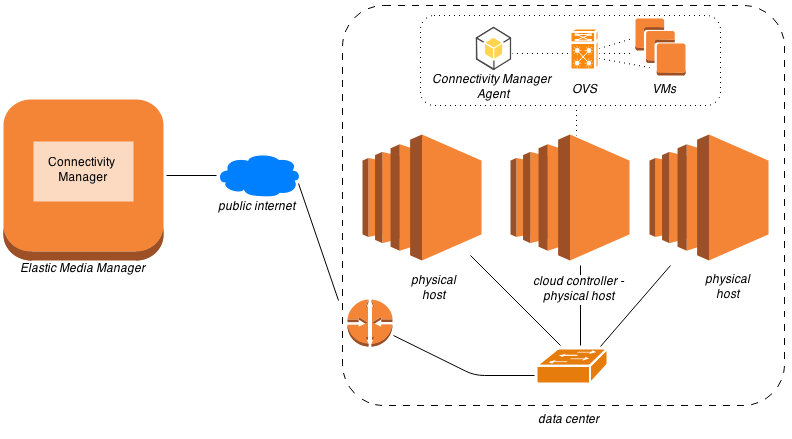
\includegraphics[width=0.8\textwidth]{images/design/scope_architecture.png}

\caption{Architectural overview}
\end{figure}

\newpage
In virtualized cloud infrastructure like OpenStack, the placement of Virtual Machines (VMs) on a particular compute node can be decided on by comparing different run-time parameters. The network connectivity between those VMs has to be prioritized and classified depending on the type of service that the server provides.

Currently there are a number of solutions for managing network connectivity between virtual servers that partially fit the requirements of this work. A comparison and their current limitations follows in the next section. The selected approach is the extension of existing network control and management services with Quality of Service (QoS) capabilities and the ability to choose a host for the deployment of the topology. In support of the thesis the Connectivity Manager will be implemented and the evaluation of the network performance will be performed on basis of the services of the NUBOMEDIA project.


\section{Overview}

\textbf{Chapter 1} begins with the motivation for this thesis and gives a brief introduction into the objectives and the scope.

\textbf{Chapter 2} gives an overview of traditional network concepts and a introduction to SDN and its components. Furthermore the different services that OpenStack consists of will be described.

\textbf{Chapter 3} conceptualizes the state-of-the-art solutions that are currently available and evaluates their implementation and limitations.

\textbf{Chapter 4} contains an analysis of requirements.

\textbf{Chapter 5} gives an architectural overview of the Connectivity Manager. Moreover design aspects are introduced and illustrated in relation to their requirements.

\textbf{Chapter 5} examines the implementation of the Connectivity Manager and Agent.

\textbf{Chapter 6} evaluates the network performance tests on the basis of one use-case.

\textbf{Chapter 7} summarizes the results of this work and gives an outlines possible future work.



\chapter{Fundamentals and Related Work}

\section{Software-Defined Networking}
The origin of Software-Defined Networking (SDN) began already in 1995, however the first use cases were only developed in 2001 and the promotion of SDN only began with the foundation of the non-profit industry consortium Open Networking Foundation (ONF) in 2011. \cite{roadtosdn}
The ONF is dedicated to push and adapt open standards like the OpenFlow into the industry.
In this following section a brief overview of the SDN architecture and concepts, including the OpenFlow protocol is given.

\subsection{Motivation}

Today's internet is part of the modern society, be it for private users, enterprises or vital infrastructure services. Networks are required to evolve in order to address the challenges that are entailed with new applications, services and a growing number of end-users.

With a more detailed view on the challenges of current networks one comes to see the following limitations: \cite{onfnewnorm}


\begin{itemize}
\item \textbf{Inability to scale}: With the expansion of data centers, networks must grow too. Configuring and managing these additional network devices comes at a high administrative effort. With the virtualization of data centers network traffic patterns becomes more and more dynamic and unpredictable. With multi-tenancy a further complication is introduced, because different end-users and services need different network performance and might require traffic steering. Such scaling and network management cannot be done with a manual configuration of the underlying infrastructure.
\item \textbf{Complexity}: In the past decades new networking protocols have been adapted by the industry. To add or move any device, multiple existing switches, routes, firewalls must be touched in order to manage protocol-based mechanisms on a device-level. With the virtualization of servers the amount of interfaces that need network connectivity and the distribution of applications over a number of virtual machines (VMs) are another demand that the current fairly static networks cannot dynamically adapt to.
\item \textbf{Inconsistent policies}: For IT to apply a network- or data center-wide policy a lot of devices and mechanisms may need to be reconfigured. Virtual Machines are created and rebuilt within no time, but if for example access or security needs to be updated, the benefits of this dynamic are subverted(?).
\item \textbf{Vendor dependence}: Standards are needed to match the requirements of the markets with the capabilities of networks and enable network operators to customize the network to specific environments.
\end{itemize}

Traditionally decisions about traffic flowing through the network are made directly by each network device, because the control logic and forwarding hardware are tightly coupled.

\subsubsection{Classical Switches \& Routers}

Packet forwarding (data plane) and routing decisions (control plane) in classical switching and routing are both within one device. In figure .. % % FIX % %
 the main components that are depicted have the following functions:
\begin{enumerate}
\item The \textbf{forwarding path} typically handles data path operations for each packet. It generally consists of Application-Specific Integrated Circuits (ASIC), network-processors or general-purpose processors that forwards frames and packets at wire speed (line-rate). Their lookup functions can be further increased with memory resources like Content Addressable Memory (CAM) or Ternary Content Addressable Memory (TCAM) to contain the forwarding information.
\item The elements in the \textbf{control plane} are based on general-purpose processors that provide services like routing and signaling protocols, including ARP, MAC Learning and forwarding tables.
\end{enumerate}

\begin{figure}[H]
\centering

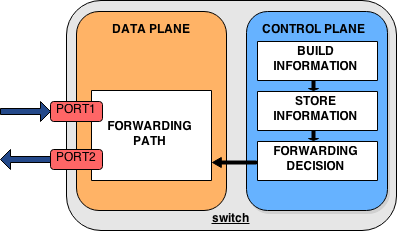
\includegraphics[width=0.5\textwidth]{images/fundamentals/switch_components}

\caption{"Classical" switch components}
\end{figure}

A switch consists of multiple ports for incoming and outgoing data. Internal forwarding tables classify the packets and forward them to one or many specific ports. It does so by collecting MAC addresses and storing their corresponding port in specific tables. Layer 2 switches also support the segregation into virtual LANs (VLAN), which enables the network operator to logically isolate networks that share a single switch.

Routers forward packets on the Network layer (Layer 3) and routing-decisions are made based on IP addresses. They contain a routing table where paths to neighbour networks are stored, so that packets can be forwarded to their destination IP address. Other features that can be configured with routers are Quality of Service (QoS), Network Address Translation (NAT) and packet filtering.

The main differences between the classical architecture and SDN will be further described in the coming sections.

\subsection{Software-Defined Networking Concept}

SDN represents a new dynamic, manageable, cost-effective and adaptable architecture \cite{onfdefinition} that is built to serve the dynamic infrastructures that are needed as a backbone for today's data centers. Opposed to the traditional approach, network control and forwarding functions are decoupled and thus can be programmed and divided into different applications and network services.
The work of the Open Networking Foundation laid out the OpenFlow protocol as the base for modern SDN solutions.

\subsection{SDN Architecture}

SDN separates the architecture into three distinct layers that communicate with each other through different APIs. In figure .. % % FIX % %
 this separation is shown.

\begin{itemize}
\item \textbf{Infrastructure Layer:} here all physical and virtual devices (e.g. switches and routers) that are capable of the OpenFlow Protocol provide forwarding mechanisms on different Network Layers.
\item \textbf{Control Layer:} represents the 'network intelligence' and collects global view of the network, by communicating with the switching elements through the so called Southbound API.
\item \textbf{Application Layer:} consists of business applications that allow the network operator to extend the SDN controller on an abstracted level, without being tied to the actual details of the implementation of the infrastructure. This communication with the Control Layer


\end{itemize}

\begin{figure}[H]
\centering

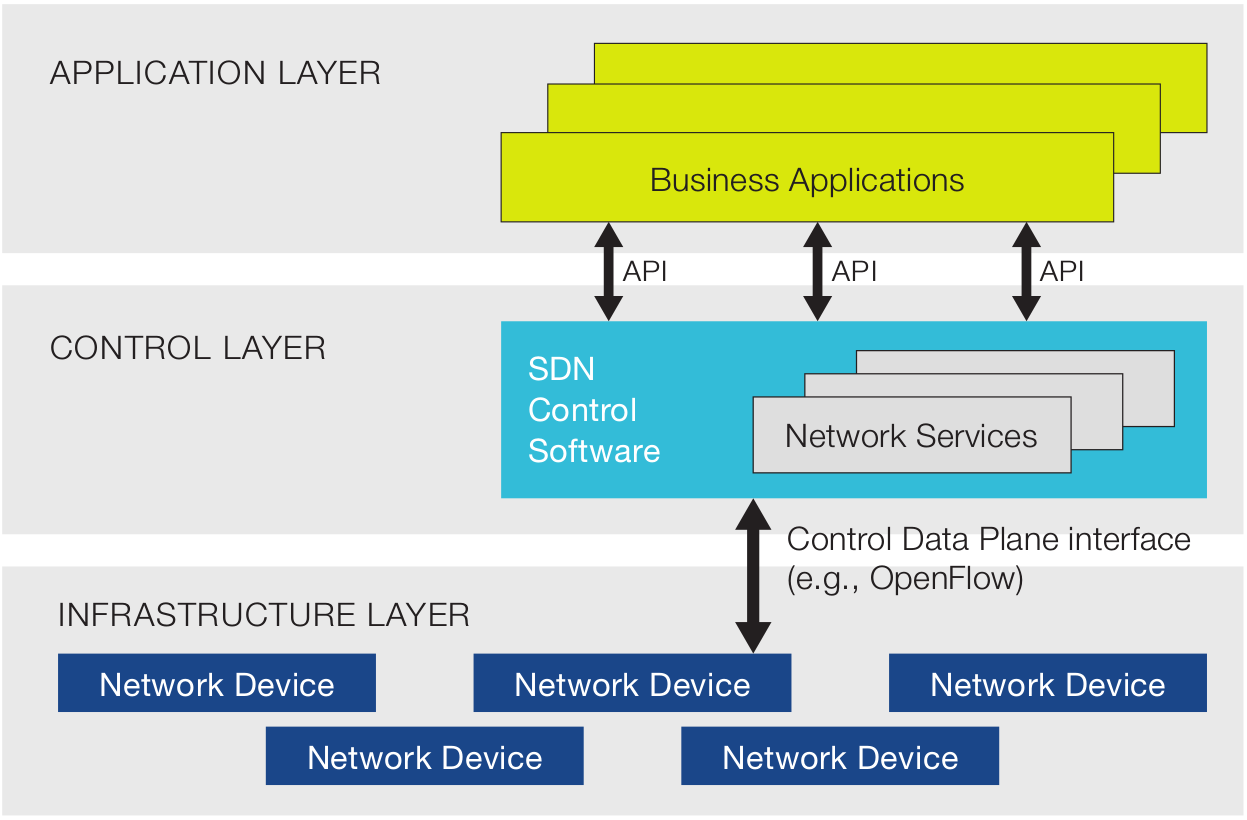
\includegraphics[width=0.5\textwidth]{images/fundamentals/sdn_logical_architecture.png}

\caption{Software-Defined Network architecture}
\end{figure}

\subsection{OpenFlow}


With OpenFlow the Open Networking Foundation defined the first standard communications interface between the SDN architecture's control and forwarding layers. It enables manipulation and direct access to the forwarding plane of physical as well as virtual (hypervisor-based) network devices such as switches and routers. \cite{onfnewnorm}

\begin{figure}[H]
\centering

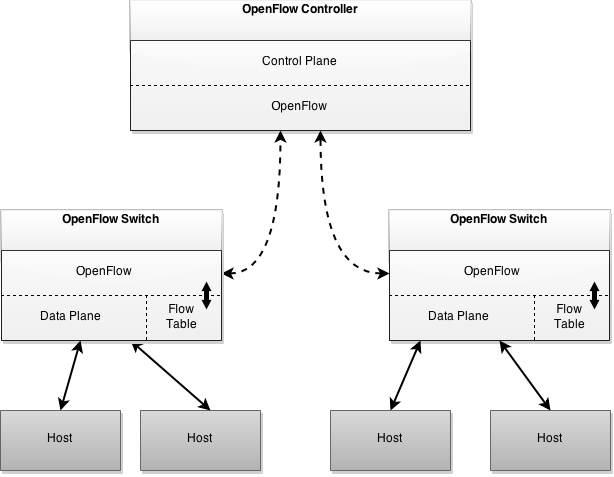
\includegraphics[width=0.6\textwidth]{images/fundamentals/openflow_architecture.png}

\caption{OpenFlow Network Architecture}
\end{figure}

OpenFlow first of all stands for the communications protocol that is used by SDN controllers to fetch information and configure switches. Additionally it is a switch specification that defines its minimum capabilities in order to support OpenFlow.


Most of the OpenFlow-enabled switches and controllers currently still only support the OpenFlow version 1.0 (released in December 2009). The newest version at this date is 1.4, however this explanation of OpenFlow will be focussed on version 1.3 since that is the most recent specification which is supported by OpenVSwitch.

The main features added since version 1.0 are among others support for VLANs, IPv6, tunnelling and per-flow traffic meters. \cite{ofversion13}

Generally the switches are backwards-compatible down to version 1.0. In the following description the focus lies on the required features of all OpenFlow capable devices, however it has to be mentioned that there is also a set of optional features.

\subsubsection{OpenFlow Controller}

The OpenFlow controller is separated from the switch and has two interfaces. The northbound interface is an API to the application layer for implementing applications that control the network. The southbound interface connects with the underlying switches using the OpenFlow protocol.

\subsubsection{OpenFlow Switch}

There are two varieties of OpenFlow-compliant switches: \cite{ofspecification}
\begin{itemize}
\item \textbf{OpenFlow-only:} in these switches all packets are processed by the OpenFlow pipeline and they have no legacy features.
\item \textbf{OpenFloy-hybrid:} support OpenFlow and normal Ethernet switching (including traditional L2 Ethernet switching, VLAN isolation, L3 routing, ACL and QoS). Most of the commercial switches that are available on the market today are this type.
\end{itemize}

An OpenFlow switch includes one ore multiple flow tables and a group table, which have the function of carrying out packet lookups and forwarding. Another component is the OpenFlow channel to the external controller \cite{ofspecification}.

\begin{figure}[H]
\centering
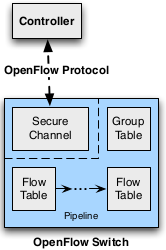
\includegraphics[width=0.3\textwidth]{images/fundamentals/openflow_switch_components.png}
\caption{OpenFlow Switch components}
\end{figure}

Through the connection using the OpenFlow protocol, it is possible for the controller to add, update and delete flow entries in flow tables.  This action can be performed either reactively or proactively. Sets of flow entries are stored in each flow table and each flow entry consists of \textit{match fields}, \textit{counters}, and a set of \textit{instructions} used for matching packets. (see OF Tables section)

The matching of flow entries begins at the first flow table, however it may continue to additional flow tables, and it uses the first matching entry from each table and performs the instruction that is linked with that specific entry. For packets without any matches a table-miss flow entry can be configured. Flow entries are usually forwarded to a physical port.

The instructions can either include actions  or modify pipeline processing. Packet forwarding, packet modification and group table processing are the possible actions. With pipeline processing packets can be permitted to be sent to other tables for further processing and metadata can be exchanged between tables.

Packets can also be directed to a group, which contains a set of actions for flooding and more complex forwarding semantics (e.g. multipath, fast reroute and link aggregation).

\subsubsection{OpenFlow Ports}
OpenFlow ports are the network interfaces used for passing packets between OpenFlow processing and the rest of the network \cite{ofspecification}.
There are various types of ports that are supported by OpenFlow. This section will give a short overview about this port abstraction.
Incoming OpenFlow packets enter the switch on an ingress port, are then processed by the OpenFlow pipeline and forwarded to an output port. (See OF Tables figure for processing).

There are three types of OpenFlow ports that must be supported by an OpenFlow switch:
\begin{itemize}
\item \textbf{Physical ports:} are hardware interfaces on a switch.
\item \textbf{Logical ports:} don't directly interact  with a hardware interface.
\item \textbf{Reserved ports:} contain generic forwarding actions (e.g. sending to the controller, flooding or forwarding using traditional switch processing)
\end{itemize}

\subsubsection{OpenFlow Tables}

\textbf{\underline{Pipeline Processing}}

The OpenFlow pipeline defines specifies how packets correspond with each of the flow tables \cite{ofspecification}. 

\begin{figure}[H]
\centering
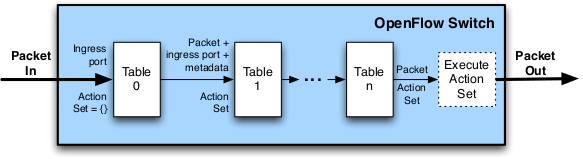
\includegraphics[width=0.8\textwidth]{images/fundamentals/openflow_pipeline_processing.png}
\caption{OpenFlow pipeline processing}
\end{figure}

As illustrated in the figure, each packet is matched against the flow entries starting at the first flow table, called flow table 0. The outcome of the match then decides if other of the sequentially numbered tables may be used. In the following sections the components of the Flow table, the matching procedures and different instructions will be described.


\textbf{\underline{Flow Table}}

A flow table contains flow entries which consist of the following fields \cite{ofspecification}: 

\begin{table}[H]
\centering

\begin{tabular}{|c|c|c|c|c|c|}
\hline Match Fields & Priority & Counters & Instructions & Timeouts & Cookie \\ 
\hline 
\end{tabular} 

\caption{Fields within a Flow table}
\end{table}

\begin{itemize}
\item \textbf{match fields:} ingress port, packet headers and optionally metadata
\item \textbf{priority:} set the priority of the flow entry
\item \textbf{counters:} is updated for matching packets
\item \textbf{instructions:} to alter the action set or pipeline processing
\item \textbf{timeouts:} set maximum amount of time or idle time before expiration of the flow
\item \textbf{cookie:} is a opaque data value chosen by the controller
\end{itemize}

Each flow table entry is uniquely identifiable by its match fields and priority. 


\underline{\textbf{Packet Matching}}

\begin{figure}[H]
\centering
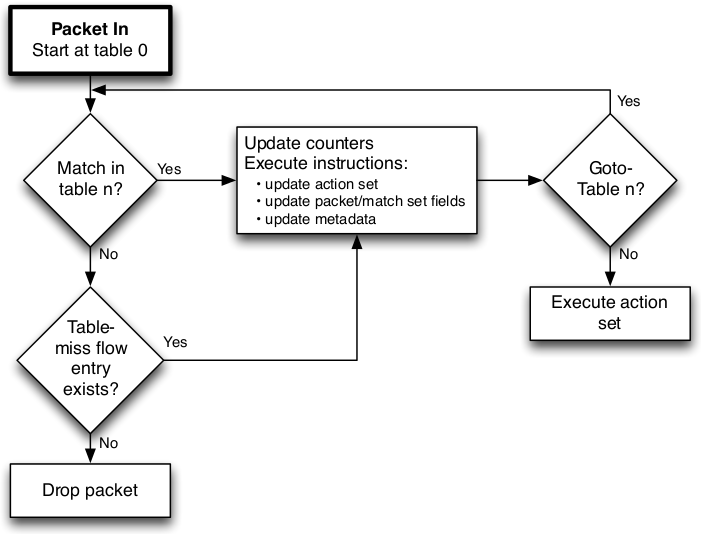
\includegraphics[width=0.6\textwidth]{images/fundamentals/openflow_packet_matching.png}
\caption{Packet flow through an OpenFlow switch}
\end{figure}

On a packet's arrival at the Flow Table, the packet match fields are extracted and used for the table lookup \cite{ofspecification}. They include different packet header fields. Additionally matches can be made against the ingress port and metadata fields.
If the values in the packet match fields equate  only the flow entry with the highest priority is selected. The associated counters are updated and the instruction set applied.

When the instruction set associated with a matching flow entry does not specify a next table, the pipeline processing stops. Only then the packet is processed with it's action set and in most cases forwarded. as shown in Figure 2.6.
However, if the lookup phase does not match any of the entries, a table-miss event occurs.


\underline{\textbf{Table-miss}}

Each flow table must support a table-miss flow entry which specifies how to process packets that are unmatched by other flow entries. The instructions associated with this entry are very alike to any other flow entries, packets are either forwarded to other controllers, dropped or it is continued with the next flow table. In case the table-miss flow entry is non-existent unmatched packets are dropped by default. 


\underline{\textbf{Group Tables}}

A group table consists of group entries and it provides a way to direct the same set of actions as part of action buckets to multiple flows. A flow entry is pointed to a group and enables additional methods of forwarding (e.g. broadcast or multicast).


\underline{\textbf{Meter Tables}}

Meters are on a per-flow level and allow OpenFlow to implement various QoS operations, such as rate-limiting, but it can also be combined with per-port queues to implement more complex QoS like DiffServ.

The main components of a meter entry in the meter table are:

\begin{table}[H]
\centering

\begin{tabular}{|c|c|c|}
\hline Meter Identifier & Meter Bands & Counters \\ 
\hline 
\end{tabular} 

\caption{Fields within a meter entry in the meter table}
\end{table}

\begin{itemize}
\item \textbf{meter identifier:} a 32 bit unsigned integer uniquely identifying the meter
\item \textbf{meter bands:} each meter band specifies the rate of the band and the action that is triggered by exceeding the limit
\item \textbf{counters:} is updated when packets are processed by the meter
\end{itemize}

The rate of packets assigned to a meter are measured and controlled. Meters are directly attached to flow entries, as opposed to queues that are attached to ports. A meter is able to have one or more meter bands, each of which specifies the rate and the way packets should be handled. If the current measured meter rate reached the rate-limit, the band applies an action. 

A meter band is identified by its rate and consists of the following fields:

\begin{table}[H]
\centering

\begin{tabular}{|c|c|c|c|}
\hline Band Type & Rate & Counters & Type specific arguments \\ 
\hline 
\end{tabular} 

\caption{Fields within a meter band}
\end{table}

\begin{itemize}
\item \textbf{band type:} defines how the packets are processed
\item \textbf{rate:} selects the meter band for the meter and defines the lowest rate at which the band can apply
\item \textbf{counters:} is updated when packets are processed by the meter
\item \textbf{type specific arguments:} some band have optional arguments
\end{itemize}

\begin{figure}[H]
\centering
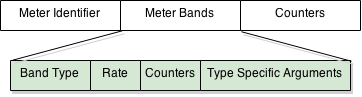
\includegraphics[width=0.6\textwidth]{images/fundamentals/openflow_qos.png}
\caption{OpenFlow QoS as a meter}
\end{figure}


\underline{\textbf{Instructions}}

Instructions are executed when a packet matches the flow entry \cite{ofspecification}. Their result is either a change to the packet, action set and/or pipeline processing. There are different instruction types and some of them are required for an OpenFlow-enabled switch whereas others are optional:

\begin{itemize}
\item \textbf{Meter \textit{meter\_id}:} direct packet to the specified meter. The packet may be discarded as the result of the metering.
\item \textbf{Apply-Actions \textit{action(s)}:} Applies the specific action(s) instantly, without any change to the Action Set.
\item \textbf{Clear-Actions:} Immediately clears all the actions in the action set.
\item \textbf{Write-Actions \textit{action(s)}:} Merges the specified action(s) into the current action set.
\item \textbf{Write-Metadata \textit{metadata / mask}:} Writes the masked metadata value into the metadata field.
\item \textbf{Goto-Table \textit{next-table-id}:} Indicates the next table in the processing pipeline.
\end{itemize}

A maximum of one instruction of each type is associated with a flow entry and they are executed in the order as specified by the given list. Flow entries can also be rejected if the switch is not able to execute its instruction.


\underline{\textbf{Action Set}}

An action set is associated with each packet, which is empty by default \cite{ofspecification}. The action set can be modified using a \textit{Write-Action} or a \textit{Clear-Action} instruction. If there is no \textit{Goto-Table} instruction within the instruction set of a flow entry the pipeline processing is halted and the actions in the action set of the packet are executed.


\underline{\textbf{Actions}}

The following action types are available on OpenFlow-enabled switches \cite{ofspecification}:
\begin{itemize}
\item \textbf{Output:} A packet is forwarded to a specified OpenFlow port.
\item \textbf{Set-Queue:} Sets the queue id for a packet. This id helps determining which queue attached to this port is used for scheduling and forwarding the packet when the packet is forwarded to a port using the output action. This forwarding behaviour allows to enable basic QoS support.
\item \textbf{Group:} Process the packet through the specified group.
\item \textbf{Push-Tag/Pop-Tag:} The ability to push/pop tags such as VLAN.
\item \textbf{Set-Field:} Modifies the values of header fields in a packet.
\item \textbf{Change-TTL:} Set the values of IPv4 TTL, IPv6 Hop Limit or MPLS TTL in a packet.
\end{itemize} 

\subsection{Open vSwitch}


\subsubsection{Concept \& Functionality}

Open vSwitch (OVS) is an open source software switch that is used in virtualized server environments. It is able to forward traffic traffic between Virtual Machines (VMs) and the physical network, as well as between different VMs on the same physical host. It can be controlled using OpenFlow and the OVSDB management protocol. It can run on any Linux-based virtualization platform i.e. KVM, VirtualBox, XEN, ESXi and is part of the mainline kernel as of Linux 3.3 but can run on kernel 2.6.32 and newer \cite{ovs-faq}.

OVS supports the following features \cite{ovs-readme}:
\begin{itemize}
\item 802.1Q VLAN model
\item Link Aggregation Control Protocol (LACP)
\item GRE and VXLAN tunneling
\item fine-grained QoS control
\item OpenFlow
\item per VM interface traffic policing
\item High-performance forwarding using a Linux kernel module
\end{itemize}

The internals of OVS are as follows \cite{prognetworkingovs}:

\begin{figure}[H]
\centering
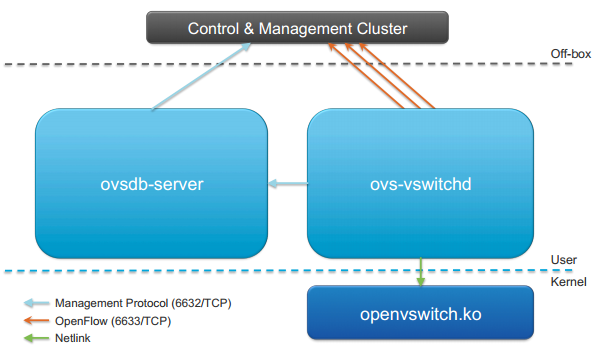
\includegraphics[width=0.6\textwidth]{images/fundamentals/openvswitch_architecture.png}
\caption{Architecture of Open vSwitch: divided into kernelspace and userspace}
\end{figure}

ovs-vswitchd, a daemon that implements the switch, along with a companion Linux kernel module for flow-based switching.
ovsdb-server, a lightweight database server that ovs-vswitchd queries to obtain its configuration.

The daemon which implements the switch is \textit{ovs-vswitchd} and is shipped with an additional Linux kernel module for flow-based switching that it communicates with using the netlink protocol \cite{ovsdeepdive}. The configuration for the switch is queried from a lightweight database server named \textit{ovsdb-server}.
Generally the decision about how a packet is processed is made in userspace, yet all following packets hit the cached entry in the kernel.

It is also possible to run it completely in userspace, but it decreases the performance drastically.


\subsubsection{OVSDB}

Each Open vSwitch daemon has a database (OVSDB) that holds it's configuration \cite{ovsdbmanual}. The database is divided into multiple different tables with different purposes, with the ones related to this project outlined below:
\begin{itemize}
\item \textbf{Open\_vSwitch}: Open vSwitch configuration
\item \textbf{Port}: Port configuration
\item \textbf{Interface}: A physical network device within a Port
\item \textbf{QoS}: Quality of Service configuration
\item \textbf{Queue}: QoS output queue
\item \textbf{Controller}: OpenFlow controller configuration
\item \textbf{Manager}: OVSDB management connection
\end{itemize}


\subsubsection{Open vSwitch Management}

Multiple different configuration utilities exist for OVS, however only ovs-vsctl is explained in this section. It is used for querying and updating the configuration of the switch through interaction with the ovsdb-server.

\begin{figure}[H]
\centering
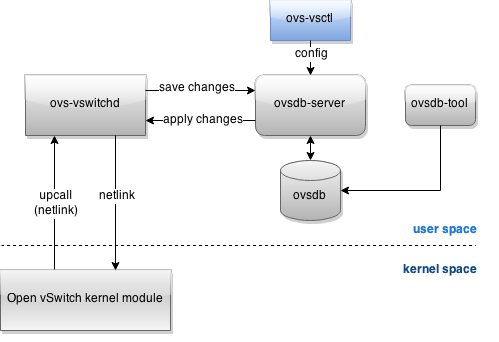
\includegraphics[width=0.6\textwidth]{images/fundamentals/openvswitch_vsctl.png}
\caption{Visualization of the interaction of the ovs-vsctl tool}
\end{figure}

Even the tool configures ovs-vswitchd, it can be seen as a high-level interface for the database.
The commands below are available for the basic OVS configuration that is needed to get it running for virtual network services:
\begin{itemize}
\item ovs-vsctl add-br \%bridge\%
\item ovs-vsctl list-br
\item ovs-vsctl add-port \%bridge\% \%port\%
\item ovs-vsctl list-ports \%bridge\%
\item ovs-vsctl get-manager \%bridge\%
\item ovs-vsctl get-controller \%bridge\%
\item ovs-vsctl list \%table\%
\end{itemize}


\subsubsection{QoS}

With Open vSwitch QoS can be configured for ports or the so-called virtual network interfaces that virtual machines get when they are connected to the internal bridge of the switch. The minimal and maximal rate-limits are defined in bytes and applied to a queue, which operates as egress shaping. The QoS port policies make use of the 'tc' implementation that is included in the Linux kernel.

\begin{figure}[H]
\centering
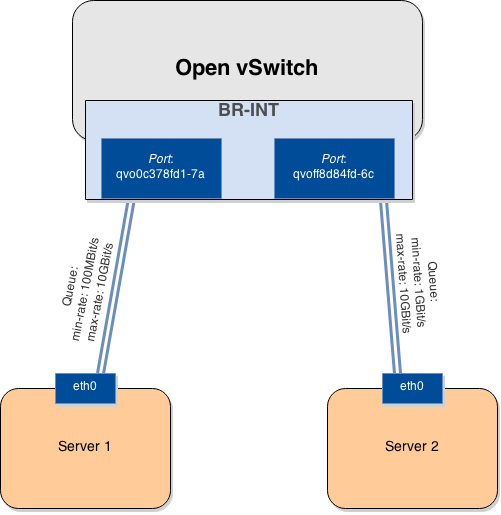
\includegraphics[width=0.5\textwidth]{images/fundamentals/openvswitch_qos-queues.png}
\caption{QoS Queues attached to a Port in OVS}
\end{figure}


% % http://linux.die.net/man/8/tc % %
% % http://linux.die.net/man/8/tc-htb % %
% % http://www.istudies.net/journal/sites/default/files/Extended%20Linux%20HTB%20Queuing%20Discipline%20Implementations.pdf % %
% %https://github.com/stanzgy/nova-network-qos/blob/master/nova-network-qos-intro.rst % %
% %http://luxik.cdi.cz/~devik/qos/htb/manual/userg.htm % %
Traffic control (tc) uses 'queuing discipline' (qdisc) for configuring the network interface \cite{tc-manual}. They are the fundamental schedulers used under Linux. When a packet is sent, it is enqueued to the qdisc for the interface and shortly after the kernel is trying to get as many packets as it can from the qdisc, so they can be forwarded to the network adaptor driver. By default the 'pfifo\_fast' qdisc is set in the kernel, which is a pure 'First In, First out' queue.

When setting QoS in OVS a classful qdisc named Hierarchy Token Bucket (HTB) is used. HTB is meant as a more understandable, intuitive and faster replacement for the Class Based Queuing (CBQ) qdisc in Linux \cite{htb-guide}. It helps to control the use of the outbound bandwidth on a given link. 


\subsubsection{GRE}

Generic Routing Encapsulation (GRE) is used in OpenStack to tunnel the traffic between multiple nodes \cite{gre-juniper}. It provides a private and secure path by encapsulating data packets.


\section{Cloud Computing Infrastructures}
% Call it Infrastructure-as-a-Service? %


\subsection{OpenStack}

The OpenStack project was founded by Rackpace Cloud and NASA, however currently more than 200 companies are contributing.
With OpenStack one is able to design, deploy and maintain a private or public cloud. It is a flexible, scalable and open-source approach that combines multiple technologies into one Infrastructure-as-a-Service (IaaS) \cite{openstack-ops}. All of the interrelated services include an API that offers administrators different ways of controlling the cloud, be it through a web interface, a command-line client or a software development kit. All of the core components that come with OpenStack are implemented in Python.


\textbf{Conceptual architecture}


The following graph shows the interaction between different OpenStack services that are involved in launching a virtual machine.

\begin{figure}[H]
\centering
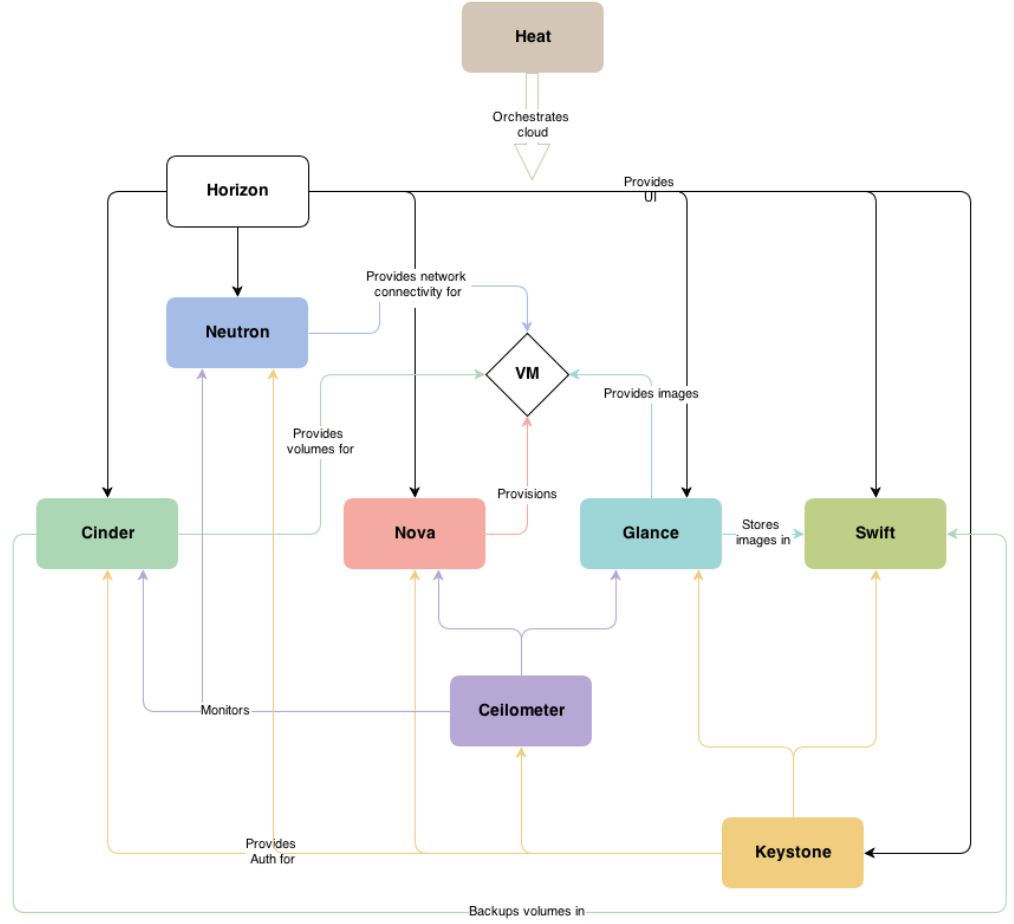
\includegraphics[width=0.8\textwidth]{images/fundamentals/openstack_conceptual_arch.png}
\caption{Interaction among OpenStack services}\cite{openstack-installjuno}
\end{figure}


\subsection{OpenStack Compute (Nova)}

Nova is used to host and manage cloud computing systems. It supports different hypervisors and the number of physical hosts running the compute services can be scaled horizontally with no requirement of hardware resources from specific vendors. Hosts that provide Nova services are also called 'Compute Nodes'. Data center can be divided into so called tenants, which are isolated users with their own servers, security groups and externally reachable IP addresses (Floating IP addresses). 

\begin{figure}[H]
\centering
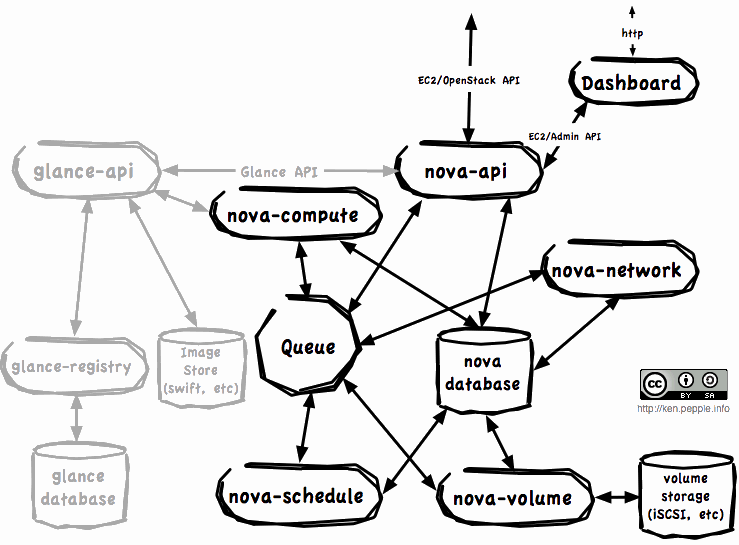
\includegraphics[width=0.5\textwidth]{images/fundamentals/openstack_nova.png}
\caption{OpenStack Compute service}
\end{figure}

\textbf{Compute Node segregation}

An OpenStack cloud can be logically and physically grouped on different levels \cite{openstack-ops}:
\begin{itemize}
\item \textbf{Region:} A Region has its own full OpenStack deployment and can be physically at a different location. Regions share a set of Keystone and Horizon services to provide access control and the graphical management interface.
\item \textbf{Availability Zone:} Inside of a Region, it is possible to logically group multiple compute nodes into Availability Zones. This zone can be specified when new servers or stacks (via Heat) are instantiated.
\item \textbf{Host Aggregates:} Compute nodes can also be logically grouped into Host Aggregates by using meta-data to tag them. This feature can be used to separate nodes with certain hardware characteristics (e.g. with SSD drives) from others.
\end{itemize}

For zoning compute nodes availability zones will be used in the Connectivity Manager in order to achieve the best networking performance between individual servers.


\subsection{OpenStack Orchestration (Heat)}

Heat provides a template-based orchestration service for creating and managing cloud resources. This means multiple OpenStack resource types (such as virtual machines, floating IP addresses, volumes, security groups and users) can be generated and also maintained with additional functionality like auto-scaling.



\subsection{OpenStack Neutron}
% % PDF: Performance of Network Virtualization in CCI % %

In the early versions of OpenStack, virtual networking was a sub-component of Nova called Nova-network. This service had it's limitations, because it was closely coupled with networking abstractions and there were no APIs available. With Neutron the implementation is decoupled from the network abstraction and it provides a flexible management interface to administrators and users.


\subsubsection{Networking Concepts}


Neutron is responsible for defining network connectivity and addressing within OpenStack. In the main network abstraction the following components are defined. A network as a virtual layer 2 segment, a subnet as a layer 3 IP address space used within a network, a port as an interface to a network or subnet, a router that performs address translation and routing between subnets, a DHCP server responsible for IP adress distribution, a security group for filtering rules acting as a cloud firewall and Floating IPs to give VMs external network access.

Neutron exposes an extensible set of APIs for creating and managing those. Neutron consists of the following elements \cite{openstack-training}:
\begin{itemize}
\item \textbf{neutron-server:} Provides the logic for SDN and does not contain any SDN functionality in itself. It provides a generic API for the network operations, is modular and extended with the following agents.
\item \textbf{L2 agent:} Plugin-specific agent that manages networking on a compute node. For more details, see ML2 section.
\item \textbf{DHCP agent:} Provides DHCP services to tenant networks through dnsmasq instances.
\item \textbf{L3 agent:} Provides L3/NAT forwarding to allow external network access for VMs (virtual routers).
\item \textbf{Metadata agent:} Acts as a proxy to the metadata service of Nova
\end{itemize}

The different agents can interact with the neutron-server process through RPC and the OpenStack Networking API. In most use-cases the neutron-server and the different agents can run on the controller node or on a separate network controller node, however the plugin agent is running on each hypervisor.


\subsubsection{Modular Layer 2}

The ML2 plugin is a framework that allows the simultaneous usage of multiple layer 2 networking technologies.

\begin{figure}[H]
\centering
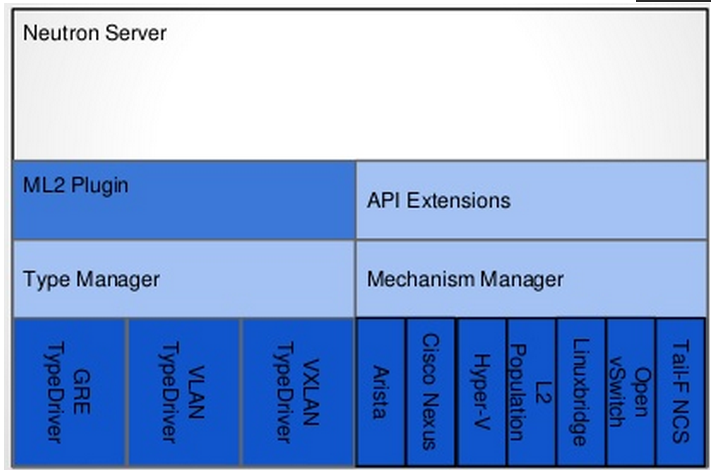
\includegraphics[width=0.5\textwidth]{images/fundamentals/neutron_ml2.png}
\caption{Neutron modular framework, including ML2 drivers}
\end{figure}

The plugin interfaces with the type driver and the mechanism driver. The type driver defines the network types that can be declared when a new network is created and currently includes: local, flat, vlan, gre and vxlan. The mechanism driver specifies the mechanism for accessing these networks, i.e. Open vSwitch, Linux Bridge or other vendor-specific solutions. 



\textbf{ML2: Open vSwitch}

Open vSwitch is the ML2 mechanism driver that is set as default when installing using Devstack and is also the most commonly deployed agent.

% % Recreate this graphic!! % %
% % alternatively use neutron_gre_connection.png from http://docs.openstack.org/openstack-ops/content/network_troubleshooting.html % %
\begin{figure}[H]
\centering
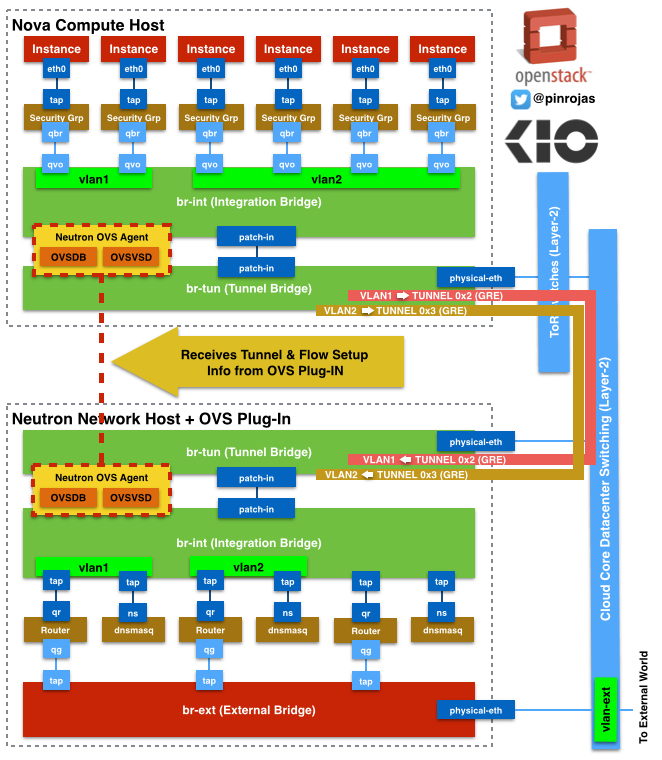
\includegraphics[width=0.5\textwidth]{images/fundamentals/neutron_gre_connection_nodes.jpg}
\caption{GRE tunneling between Controller Node and Compute Node}
\end{figure}

\subsubsection{Network Distinction}

Neutron is connected to different networks. For internet routable connections the external network is used. The management network is created by the network operator and is mapped to pre-existing networks within the datacenter, which is used to connect the different hosts. The tenants within OpenStack have their own isolated self provisioned private networks. Those can optionally be connected to other tenant or external networks. The abstraction of those tenant networks is possible through network namespaces. This allows overlapping IP addresses within the datacenter.


\subsubsection{Neutron Workflow}

The workflow for Neutron, from starting to booting VMs is as follows:
\begin{enumerate}
\item Start Neutron-Server
\item Start Open vSwitch Agent
\item Start L3-Agent
\item Start DHCP-Agent
\item Start Metadata-Agent
\item Create Networks
\item Create Routers
\item Boot VMs
\end{enumerate}


\textbf{Neutron - Nova interaction}

\begin{enumerate}
\item Request: Create VM connected to network X (API)
\item Create VM (RPC: Nova API to Nova conductor)
\item Nova schedules VM
\item Create VM (RPC: Nova conductor to Nova compute)
\item Create Port (API: Nova compute to Neutron service)
\item Create tap device
\item Notify L2 agent (RPC)
\item get\_device\_details (RPC: L2 agent to Neutron service)
\item Configure local VLAN, OVS flows
\item Send port\_up notification (RPC: L2 agent to Neutron service)
\item Send port\_up notification (API: Neutron service to Nova)
\item port\_up (RPC: Nova service to Nova compute)
\item Nova compute boots VM

\end{enumerate}


\section{Conclusion}
\chapter{Requirements}

\section{Functional Requirements}

This section identifies the functional requirements of the Connectivity Manager, specifically as needed for the NUBOMEDIA use-case.

\subsection{Service-Level Agreement Enforcement}

One of the key objectives of the Connectivity Manager is to grant different Service-Level Agreements (SLA) to the links between Virtual Machines. The agreement is set as Quality of Service assurances with the minimal and maximum bandwidth rate set. Network performance problems can provide a negative experience for the end-user, as well as productivity and economic loss. This is why some services need to have an ensured premium traffic.

\subsection{Optimal Virtual Machine Placement}

The placement of Virtual Machines makes a tremendous difference in terms of connectivity and resource performance. VMs that run on the same Compute Node have a better connectivity then ones that need to communicate over wire. The fact that the networking is virtualized besides the virtualized computing environment means that a more utilized Compute Node will also have less resources available for switching and routing. A part of the motivation for this requirement can be found in the Evaluation section.

\subsection{Integration with Elastic Media Manager}

The Connectivity Manager needs to integrate with the Elastic Media Manager (EMM) which is used for deploying a topology of resources within a cloud infrastructure. Furthermore it provisions the instances and manages them during their runtime for services like upscaling the amount of instances after utilization alarms are triggered. The CM communicates with the EMM in order to enable the two previously-mentioned requirements for the overall platform.

\section{Non-functional Requirements}

Non-functional requirements generally specify criteria to do with the operation of a system and not with it's behavior. Thus the Connectivity Manager should also fit the following characteristics.

\subsection{Scalability}

Today's data-centers can grow in a fast-pace, especially in connection with automated up-scaling of compute resources at a certain level of utilization. This is why the underlying virtualized network software needs to be scalable too.

\subsection{Modularity}

Building modular software not only simplifies further development for a third-party, but also makes it easier to exchange certain parts of the software for improvements or maintenance. The separation into two different components with a defined API makes it more flexible.

\subsection{Interoperability}

In the case of the use of Open vSwitch, interoperability is given because it is made available for various architectures. The integration into the Linux Kernel and the use of standardized protocols such as OpenFlow are a significant factor.
\chapter{State of the Art}

\section{Overview}

Three existing solutions for extending the services that Neutron provides with additional SDN features have been tested. They were selected based on the requirements given in the previous section.

\section{OpenDaylight SDN Controller}


OpenDaylight is fully implemented in Java. OpenDaylight exposes a single common OpenStack Service Northbound API which exactly matches the Neutron API. The OpenDaylight OpenStack Neutron Plugin simply passes through and therefore pushes complexity to OpenDaylight and simplifies the OpenStack plugin. The ML2 mechanism driver in Neutron has to be set to the OpenDaylight ML2 plugin, with the ODL agent running on the Compute Nodes. The OpenDaylight controller can be run on the Control Node or on a separate VM \cite{odl-intro}. The Open vSwitch database (OVSDB) Plugin component for OpenDaylight implements the OVSDB management protocol that allows the configuration of Open vSwitches. The OpenDaylight controller uses the native OVSDB implementation to manipulate the OVSDB. The component comprises a library and various plugins. The OVSDB protocol uses JSON/RPC calls to manipulate a physical or virtual switch that has OVSDB attached to it \cite{odl-ovsdb}.

\begin{figure}[H]
\centering
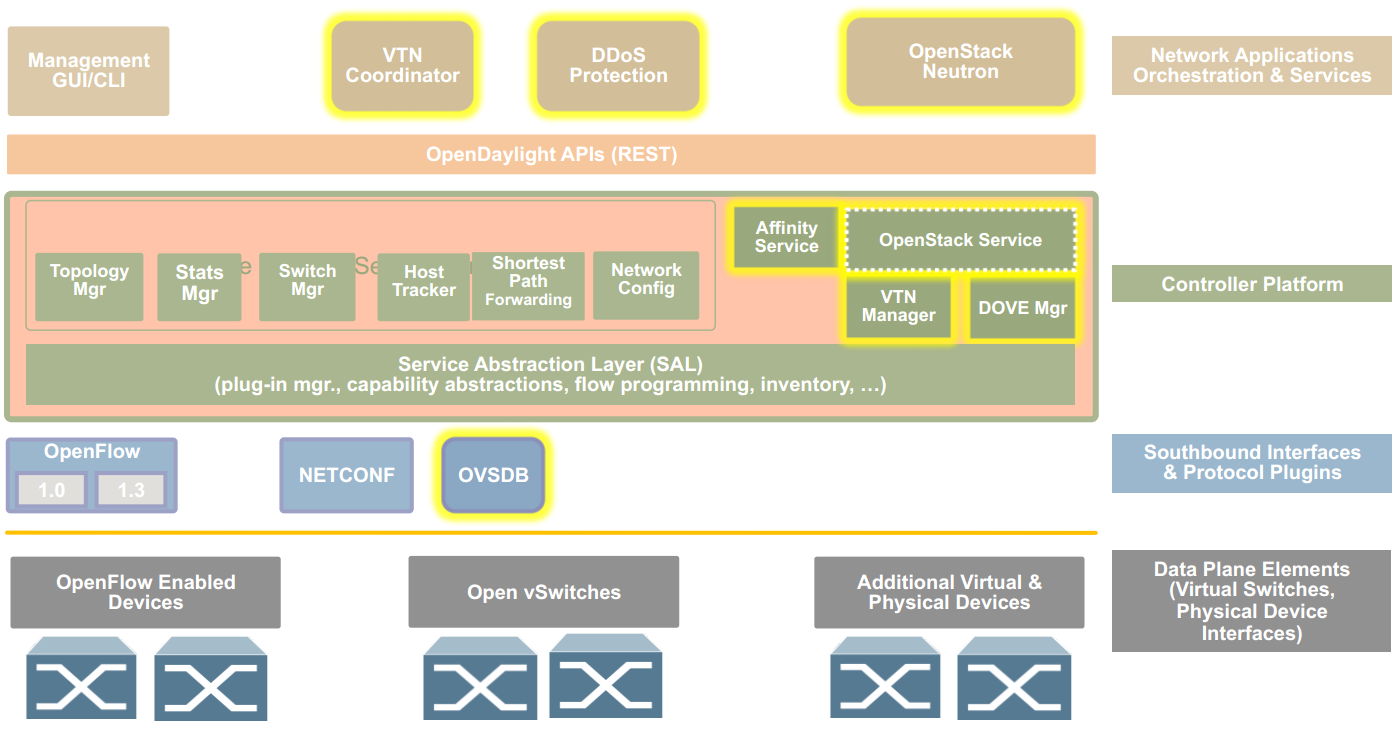
\includegraphics[width=0.9\textwidth]{images/sota/odl_architecture.png}
\caption{Architecture of OpenDaylight Virtualization edition}
\end{figure}

The OVSDB component is accessible through a Northbound ReST API, which enables the operator to connect to the OpenFlow controller and modify various OVSDB tables. Through this API QoS rules can be deployed. Because it connects directly to the OpenVSwitch tables, all the QoS types that come with OpenVSwitch can be deployed (DSCP marking, setting priority, min-/max-rate for virtual network ports within OpenFlow Queues). In the local testbed it was possible to successfully deploy QoS rules on the ports of Virtual Machines. 


\section{Ryu SDN Controller}

Ryu is a component-based software defined networking framework which fully supports OpenFlow 1.0, 1.2, 1.3 and 1.4 switches and is fully written in Python \cite{ryu-start}. Ryu is a full featured OpenFlow controller that supports GRE and VLAN tunnelling. The OpenFlow controller that is embedded in the agent sets Flows on the switch by sending OpenFlow messages to the switch \cite{ryu-comparison}. It includes a set of apps which build the base of the SDN controller: L2 switch, ReST interface, topology viewer and tunnel modules. Ryu also includes an app that allows to set QoS rules through a ReST interface which uses a OVSDB interaction library to apply those. The QoS rules can be either applied to a specific Queue within a VLAN or a Switch port. It supports DSCP tagging and setting the min-rate and max-rate of an interface.

\begin{figure}[H]
\centering
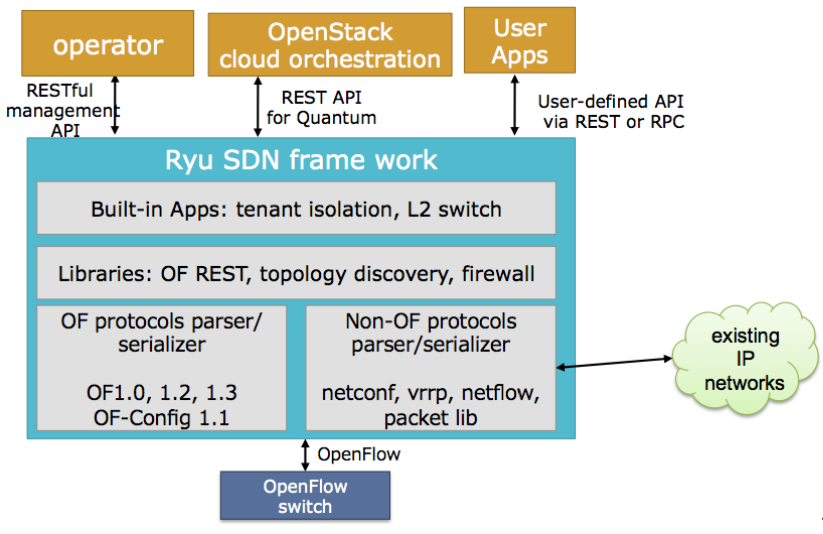
\includegraphics[width=0.7\textwidth]{images/sota/ryu_architecture.png}
\caption{Ryu architecture}
\end{figure}


As of OpenStack IceHouse Ryu makes use of the OFagent and is included in the Neutron core git repository. In order to use it as the SDN framework within Neutron, the OFagent  has to be set as both the ML2 mechanism driver (running on the control / network node) and the Neutron agent (running on the compute node). 


\section{OpenStack Neutron - QoS Extension}

A Neutron extension has been partially implemented for OpenStack IceHouse which includes an API for setting QoS on a per-tenant and per-port basis in combination with the Open vSwitch agent \cite{neutron-qos}. This approach makes a lot of sense as it extends the already existing Neutron API and the framework that is given for custom Neutron Extensions.

% -> further describe the structure of the implementation !! %

\begin{figure}[H]
\centering
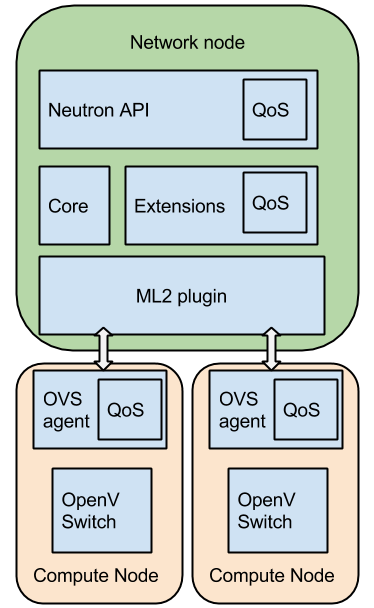
\includegraphics[width=0.3\textwidth]{images/sota/neutron_qos_extension.png}
\caption{Neutron QoS Extension architecture}
\end{figure}



\section{Problem Statement}

%Show why previously mentioned projects fail for our requirements, analyse and compare them. Make table with features. Also state that they wouldn't include the VM placement feature. %
This section lists the restrictions that have been discovered with the previously mentioned solutions. 


\textbf{Problems encountered with OpenDaylight:}

The local testbed used for the integration of OpenStack Juno and OpenDaylight Helium consisted of 2 hosts, one running the OpenStack control node and OpenDaylight Controller and a OpenStack Compute Node on the second host. During the tests it was not possible to get the public network access for the Virtual Machines working, thus the L3 routing did not work. This and the fact that it ODL is very complex to debug and understand all underlying processes led us to the decision not to use OpenDaylight.


\textbf{Problems encountered with Ryu:}

The test of Ryu was unsuccessful due to a number of errors while stacking the test environment using Devstack. It was not possible to launch instances and test the QoS features. The lack of proper documentation for the interaction with OpenStack Neutron led us to look more into other SDN controllers for our particular use case. Currently Ryu doesn't support the Distributed Virtual Routing feature that has been introduced with OpenStack Juno.


\textbf{Problems encountered with Neutron QoS Extension:}

The implementation has not been finished and merged into Neutron, however the basic deployment of QoS seem to have been tested successfully. 

At the moment it is not clear if the OpenStack community will keep working on this. According to the code review comments, it was deferred to Juno, but it is not included in the current release and no active development is stated in the code / documentation platforms of the OpenStack community.

The patch consists of an extension to the Neutron API which allows setting QoS rules through the Neutron Python client, the actual Neutron extension with the QoS, QoS Driver in the Open vSwitch agent and an addition to the Neutron Database that includes QoS.

For the scope of this work, extending Neutron with QoS is not within the time frame of the project.

\section{Conclusion}

The listed problems further strengthen the motivation for the implementation of the Connectivity Manager. Additionally, the second major requirement for the Optimal Virtual Machine Placement are not given in any of the outlined solutions. The following table lists a comparison and analysis of their features:




\begin{table}[H]
\centering

\begin{tabularx}{\textwidth}{ |X|X|X|X| }
\hline Tool/Solution & QoS support & OF Controller & OpenStack (Juno) integration \\ 
\hline Ryu & X & X & No (tests in Juno failed) \\ 
\hline OpenDaylight & X & X & No (tests in Juno failed) \\ 
\hline Neutron QoS extension & not fully implemented & No & No (IceHouse patch not ported to Juno) \\ 
\hline 
\end{tabularx}

\caption{State-of-the-art: Feature comparison}
\end{table}

\chapter{Design}

\section{Architecture overview}

The Connectivity Manager is logically located between the EMM and the cloud infrastructure and provides the following two functionalities:
\begin{itemize}
\item \textbf{Optimal Instance Placement:} During the deployment of a stack an algorithm chooses where individual instances are placed within the cloud infrastructure.
\item \textbf{Service-Level-Agreement enforcement:} Depending on the services that an instance provides to the rest of the stack, certain requirements for its network performance need to be fulfilled.
\end{itemize}

\begin{figure}[H]
\centering


\includegraphics[width=0.5\textwidth]{images/design/functional_architecture}

\caption{High-level architecture of the Connectivity Manager}
\end{figure}

The \textit{Instance Placement Engine} determines if and where the instances should be deployed. It does so by comparing the current utilization and capacity of the available compute nodes within the availability zone.

The \textit{QoS Manager} enforces different QoS policies based on the type of service that the instance is grouped in. A guaranteed and maximum bit-rate for the network port of an instance can be set. This way a certain network performance can be insured.

\section{Connection between Manager \& Agent}

The Connectivity Manager and Agent are two separate applications that communicate using a ReST API. 

\begin{figure}[H]
\centering

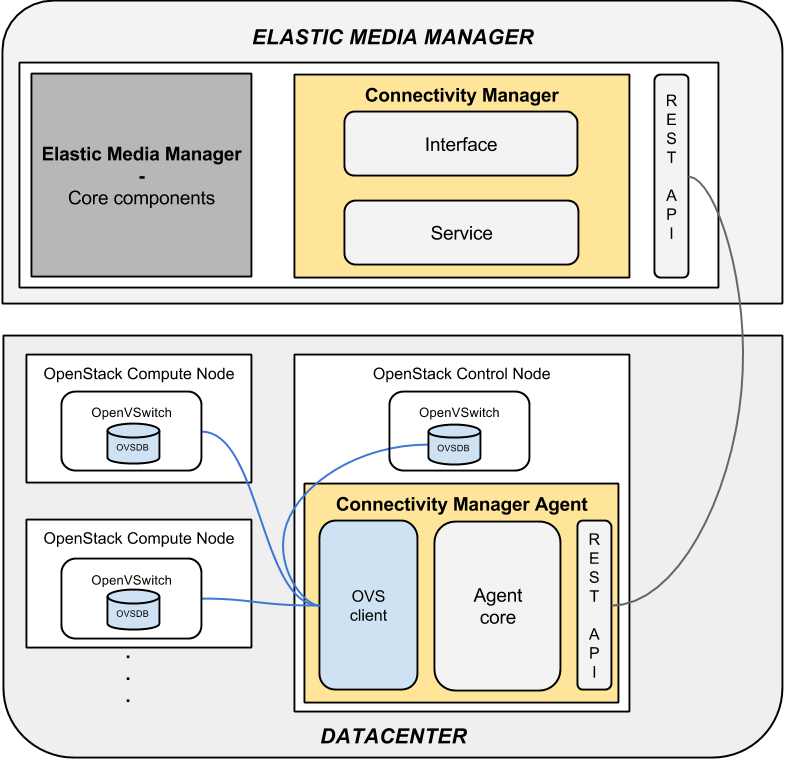
\includegraphics[width=0.6\textwidth]{images/design/modular_architecture_cm_cma}

\caption{Minimized architecture of the Connectivity Manager and its integrations}
\end{figure}

This design was chosen first of all because the Connectivity Manager is integrated in the EMM, which is required to be placed anywhere outside of the data center. Second of all the Connectivity Manager Agent needs to  the OVSDB on the compute nodes and consequently needs to be within the internal management network of the OpenStack infrastructure.

The sequence diagram below displays the work-flow that the CM passes during the run-time.

\begin{figure}[H]
\centering

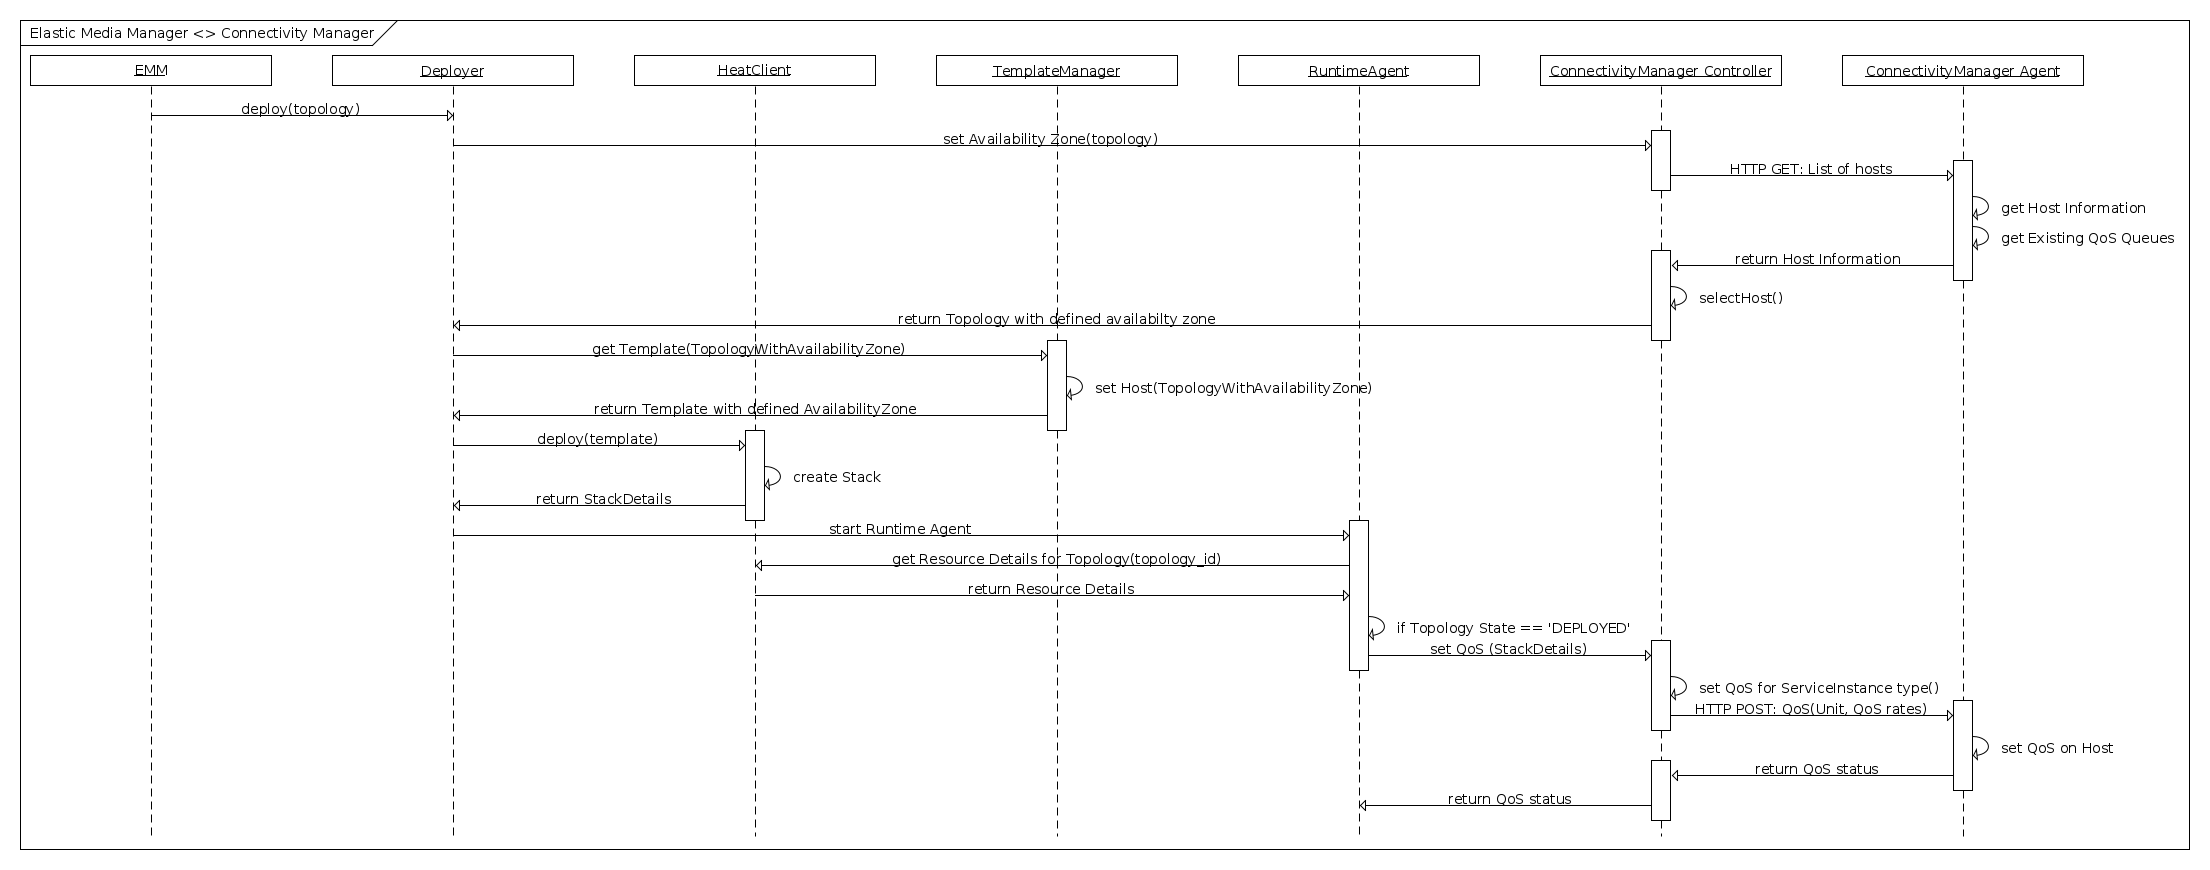
\includegraphics[width=0.9\textwidth]{images/design/sequence_diagram}

\caption{Workflow: Deployment of stack \& Assignment of QoS policies}
\end{figure}

As can be seen, the Connectivity Manager receives the Topology that contains a description of the configuration and specifications of the whole cloud. For the placement decision the CM to needs to get the information about the current state of the infrastructure. This exchange with the CM Agent occurs through the given API. Upon reception of that data, the placement algorithm sets the availability zone for each instance within the topology. The topology is then converted into a Heat template by the Template Manager. Once the template got deployed by the Heat Client a runtime agent starts. The purpose of the runtime agent is to continuously check the state of the stack. Once the stack has reached the 'DEPLOYED' state, the runtime agent requests the CM to set the QoS policies according to previously configured values. This configuration is subsequently transmitted to the CM Agent whose task is then to enable it on the according ports of the instances within the Open vSwitch.

\section{Design of Connectivity Manager}


\begin{figure}[H]
\centering

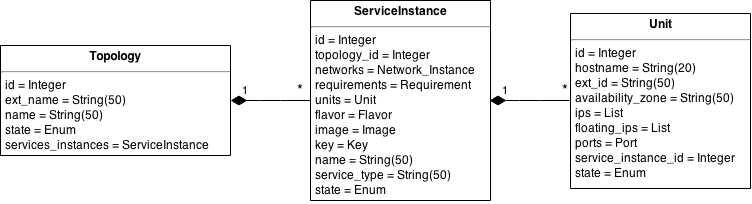
\includegraphics[width=0.9\textwidth]{images/design/cm_topology_object}

\caption{Deployment: Topology object from EMM}
\end{figure}


\subsection{Algorithm for Instance Placement}



\newpage
\section{Design of Connectivity Manager Agent}

\begin{figure}[H]
\centering

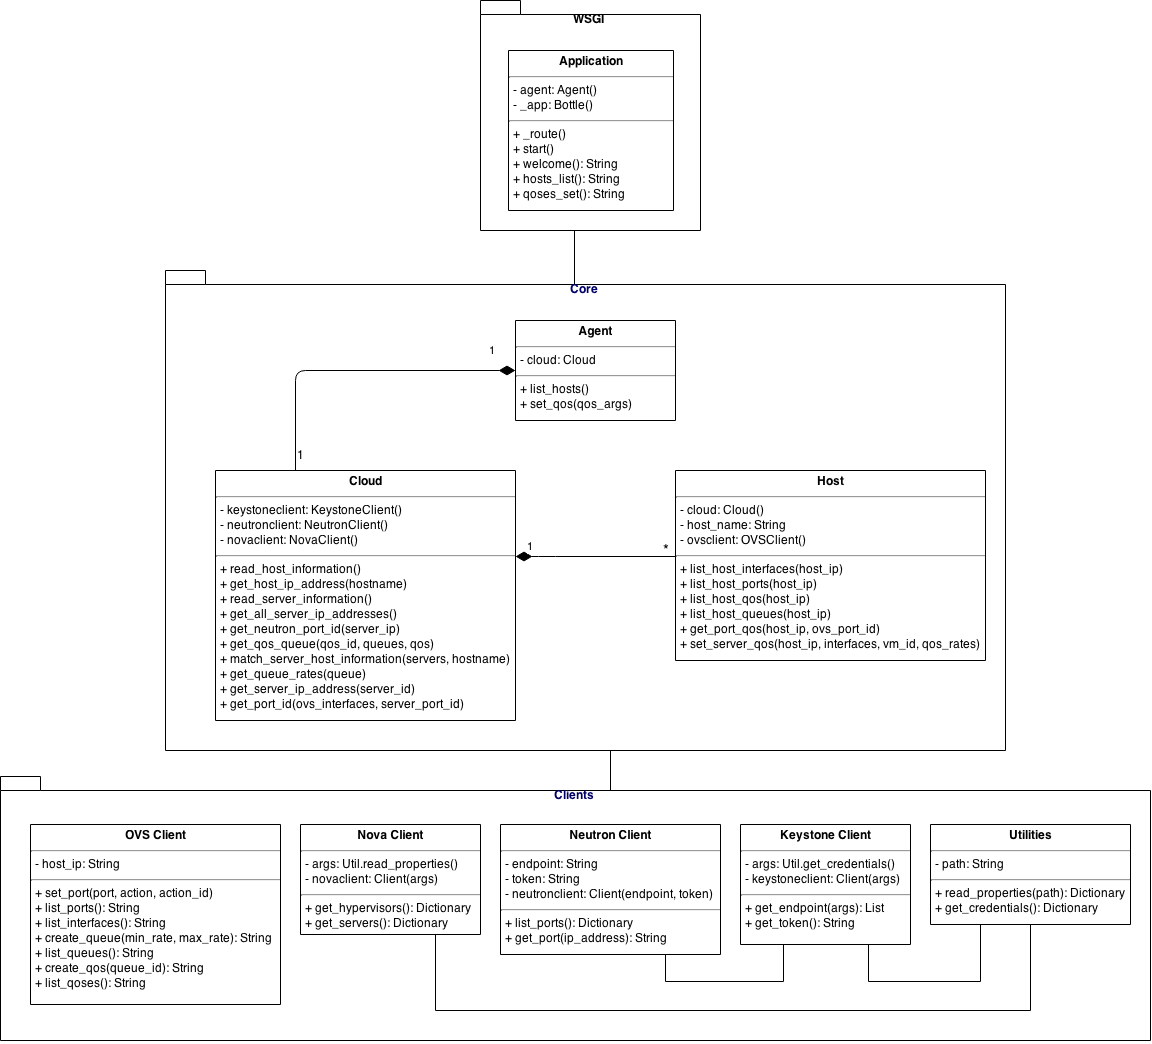
\includegraphics[width=0.7\textwidth]{images/design/cm_agent_class_diagram}

\caption{Class diagram: Connectivity Manager Agent - Core package}
\end{figure}


\begin{figure}[H]
\centering

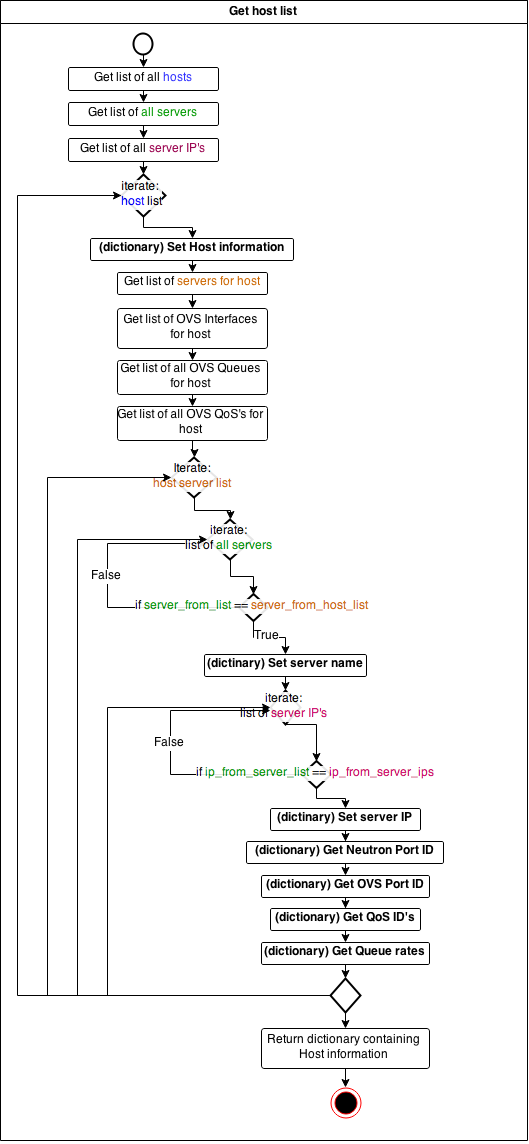
\includegraphics[width=0.7\textwidth]{images/design/activity_host_list}

\caption{Activity diagram: Get list of hosts}
\end{figure}

\begin{figure}[H]
\centering

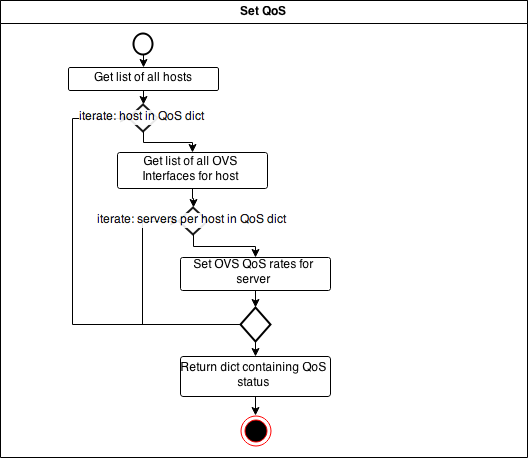
\includegraphics[width=0.7\textwidth]{images/design/activity_set_qos}

\caption{Activity diagram: Set QoS rates for all servers}
\end{figure}

\begin{figure}[H]
\centering

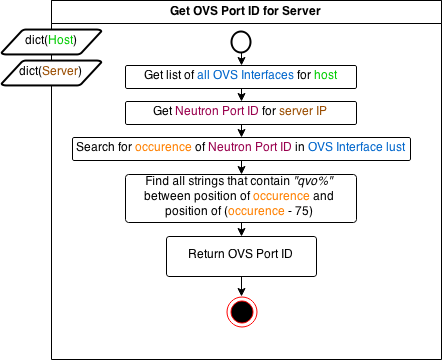
\includegraphics[width=0.7\textwidth]{images/design/activity_get_ovs_port_server}

\caption{Activity diagram: Get OVS Port ID for server}
\end{figure}

\begin{figure}[H]
\centering

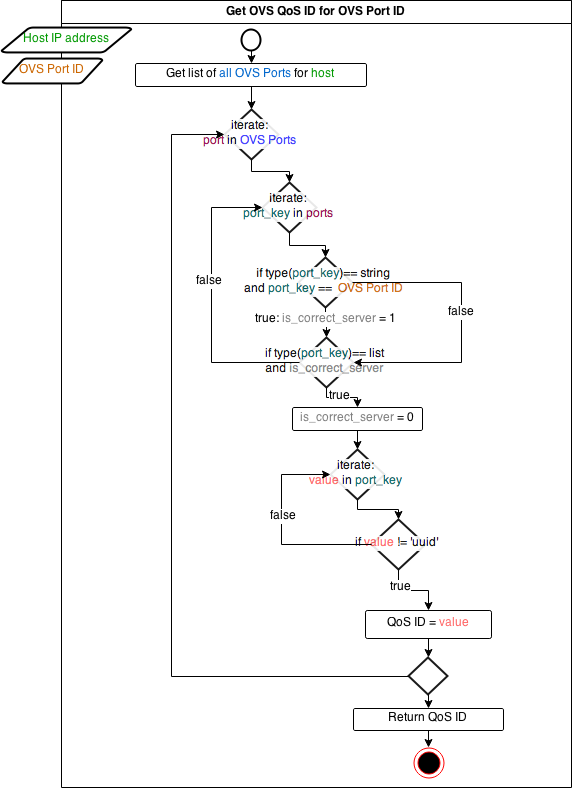
\includegraphics[width=0.7\textwidth]{images/design/activity_get_qos_id_for_ovs_port}

\caption{Activity diagram: Get QoS ID for OVS Port}
\end{figure}





\section{Conclusion}
\chapter{Implementation}


\section{Environment}

The software developed in this thesis is completely realized using the Python programming language. This choice was made because OpenStack offers Python clients that connect to their API and the Elastic Media Manager is also programmed in Python.

PyCharm was selected as the Integrated Development Environment (IDE) to simplify the programming and testing lifecycles. The code is under revision control using Git and the repository that contains both the code for the CM and CM Agent consists of two main branches: master and develop. The develop branch holds the latest changes and upon successful testing those were merged back into master, which is always in a production-ready state.

\subsubsection{Project Structure}

The code is separated into two different projects in order to allow testing of the integration concurrently. The following graphic outlines the focus within the Elastic Media Manager (EMM), whilst the CM Agent is separated and has its own structure.

\begin{figure}[H]
\centering

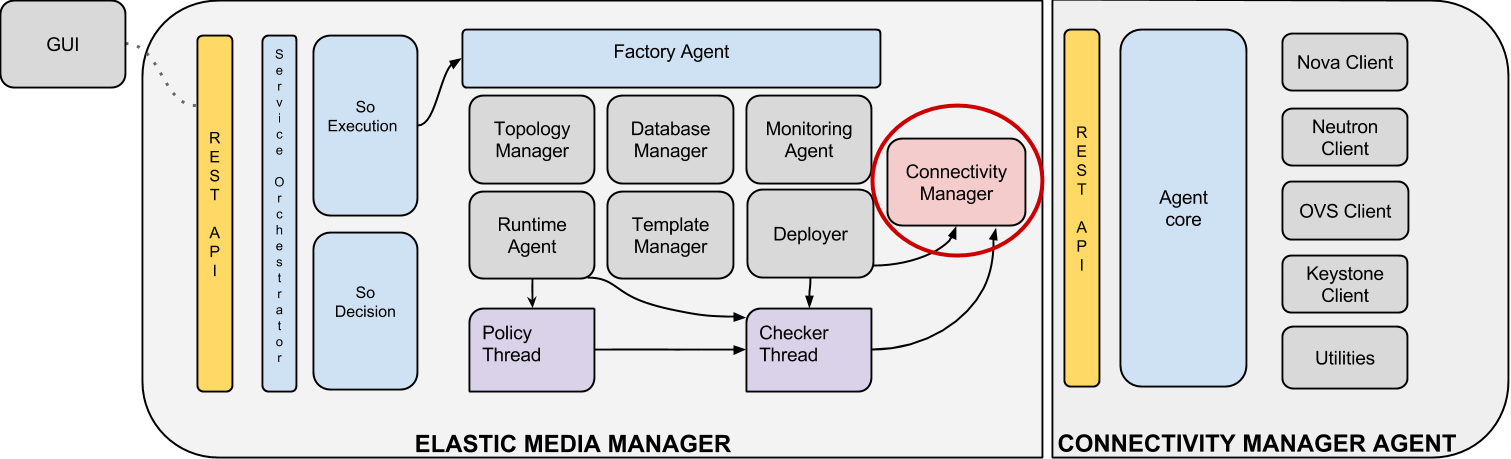
\includegraphics[width=0.9\textwidth]{images/implementation/cm_implementation_focus_overview}

\caption{Implementation focus}
\end{figure}

The structure for the CM is dictated by the already existing implementation of the EMM and the scope of this thesis includes solely its extension with a Connectivity Manager interface and service plus the needed changes in the other interfaces to make use of the methods within the CM.

The Connectivity Manager contains the ReST API, the Agent core, clients and other helper classes.

\subsubsection{Local OpenStack Test Environment}

In order to test the Connectivity Manager Agent and the use of its OpenStack API clients a test-bed was installed. This test-bed was set up using Vagrant, as it allows starting of the virtual machines from the command-line and can easily be provisioned and managed. In order to test the software across multiple compute nodes a setup with 2 VM's was installed.

For the installation of OpenStack, the devstack script was used, which takes care of not only the deployment of the different components but also their configuration. The configuration parameters are set in the 'local.conf' file. For the OpenStack cluster controller the following configuration was used:

\begin{lstlisting}[language=json]
[[local|localrc]]
ADMIN_PASSWORD=pass
DATABASE_PASSWORD=pass
RABBIT_PASSWORD=pass
SERVICE_PASSWORD=pass
SERVICE_TOKEN=a682f596-76f3-11e3-b3b2-e716f9080d50

HOST_IP=192.168.120.15
OVS_PHYSICAL_BRIDGE=br-ex
MULTI_HOST=1

# Enable Logging
LOGFILE=/opt/stack/logs/stack.sh.log
VERBOSE=True
OFFLINE=True
RECLONE=no
LOG_COLOR=True
SCREEN_LOGDIR=/opt/stack/logs

# Neutron
disable_service n-net
enable_service q-svc
enable_service q-agt
enable_service q-dhcp
enable_service q-l3
enable_service q-meta

# OpenStack API paths
MYSQL_HOST=192.168.120.15
RABBIT_HOST=192.168.120.15
GLANCE_HOSTPORT=192.168.120.15:9292
KEYSTONE_AUTH_HOST=192.168.120.15
KEYSTONE_SERVICE_HOST=192.168.120.15

IMAGE_URLS="$IMAGE_URLS,http://cloud-images.ubuntu.com/releases/trusty/
release/ubuntu-14.04-server-cloudimg-amd64-disk1.img"
\end{lstlisting}

The configuration file for the second node, which solely runs Nova, the Open vSwitch agent and the Rabbit MQ is identical except for its enabled services and host IP address:

\begin{lstlisting}[language=json]
HOST_IP=192.168.120.16
ENABLED_SERVICES=n-cpu,rabbit,neutron,q-agt,q-l3
\end{lstlisting}

During the implementation and testing phase the Connectivity Manager Agent was installed on the controller node while the EMM was executed from the local machine.

\section{Connectivity Manager - Components and Operations}

\subsubsection{Selection of Best-Performing Hypervisor}


\textbf{Step 1: Retrieve current host utilization from CM Agent}

In order to decide on the placement, the Connectivity Manager firstly needs to retrieve the host information from the Agent. It then sums up the different resource utilizations: amount of servers currently running on it, the total amount of used RAM \& vCPUs.
\begin{figure}[H]
\centering

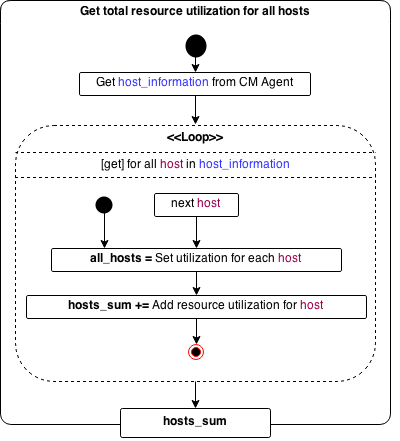
\includegraphics[width=0.4\textwidth]{images/implementation/cm_get_host_utilization}

\caption{Check resource utilization of hosts}
\end{figure}

The amount of resources that are required in total to deploy the topology on the tenant needs to be calculated by adding up the amount of resources that are needed for each Unit. This can easily be done by checking its flavor.

\begin{figure}[H]
\centering

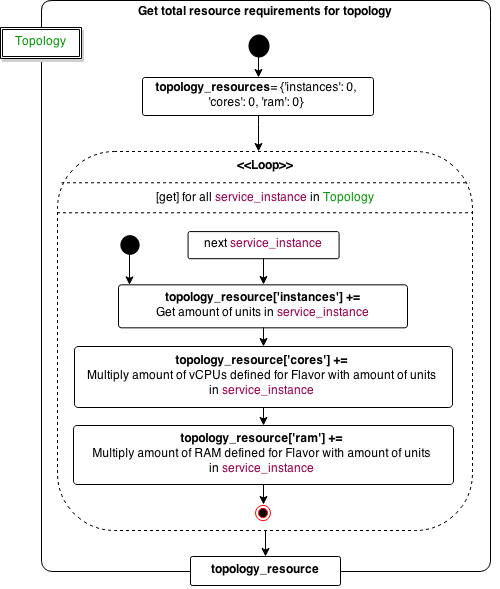
\includegraphics[width=0.5\textwidth]{images/implementation/cm_get_topology_requirements}

\caption{Get total amount of required resources for topology}
\end{figure}

\textbf{Step 2: Check if Topology is within the limitations of the Quota and currently available resources on the tenants hosts.}

In the second step it is checked if the topology is feasible for deployment. This decision is made by first comparing the values from Step 1 to the available Quota values (amount of VMs, RAM, and vCPUs required for the sum of all servers) and secondly finding out if the required resources are less or equal to the currently not utilized resources in the tenants infrastructure.

\begin{figure}[H]
\centering

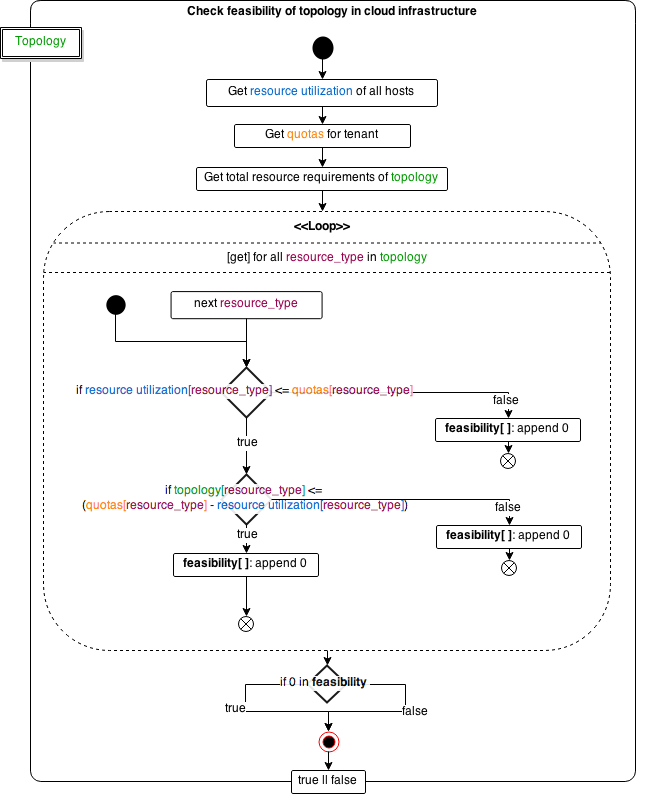
\includegraphics[width=0.6\textwidth]{images/implementation/cm_feasibility_check}

\caption{Deployment feasibility check}
\end{figure}

These comparisons need to be made, in order to conform to the requirement of not over-committing any resources.


\textbf{Step 3: Check whether the Topology can be deployed on a single host.}

The next step checks if the total amount of topology resources from Step 1 can be deployed on a single host. If there are multiple hosts that have enough capacity available, the first one within the list is returned by this method.

\begin{figure}[H]
\centering

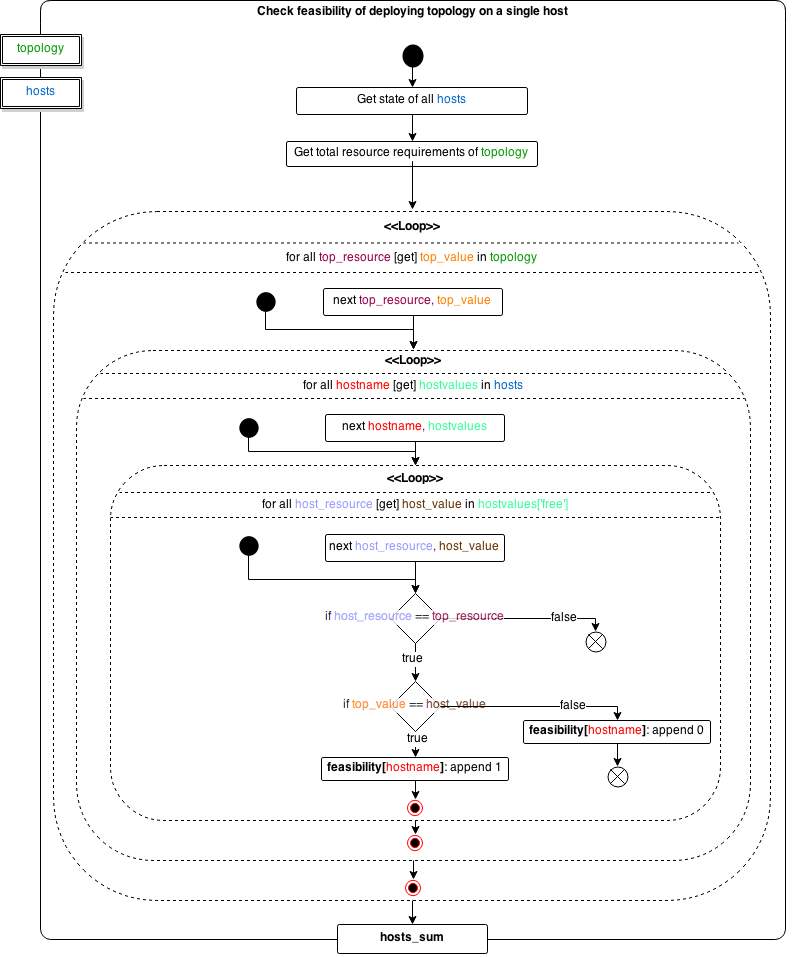
\includegraphics[width=0.7\textwidth]{images/implementation/cm_single_host_check}

\caption{Single host deployment check}
\end{figure}


\textbf{Step 4: Set selected host as availability zone for each Unit.}

Lastly the chosen host needs to be set in the topology, so it can be returned to Heat for continuing with the deployment process. The syntax for a Unit's availability zone needs the 'nova' suffix, so this string needs to be added in front of the host name.

\begin{figure}[H]
\centering

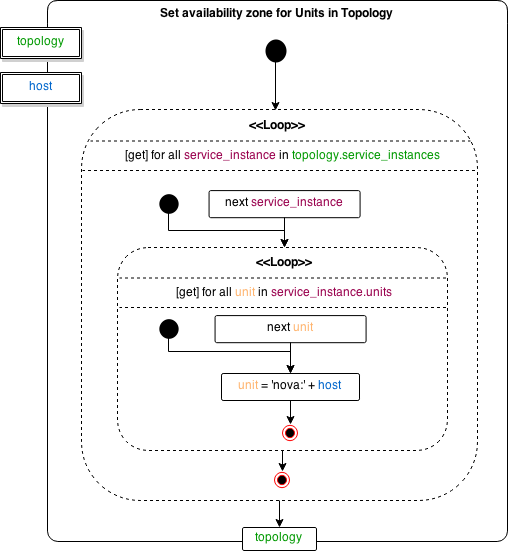
\includegraphics[width=0.5\textwidth]{images/implementation/cm_set_az_topology}

\caption{Set AZ per Unit}
\end{figure}

\subsubsection{Enabling QoS for servers}

The rates for the QoS classes can be set in the configuration of the EMM.
The default location is \textit{/etc/nubomedia/emm.properties} and it contains the following default rates:
\begin{lstlisting}[language=commands]
# CONNECTIVITY MANAGER PROPS & QOS RATES (IN BIT/S)
cm_agent_ip=192.168.41.45
# GOLD = 100MBIT/S - 10GBIT/S
gold_min=100000000
gold_max=10000000000
# WHOLESALE = 100MBIT/S - 1GBIT/S
wholesale_min=100000000
wholesale_max=1000000000
\end{lstlisting}

For setting QoS for all Units within a Service Instance, the following workflow is passed through:

\begin{figure}[H]
\centering

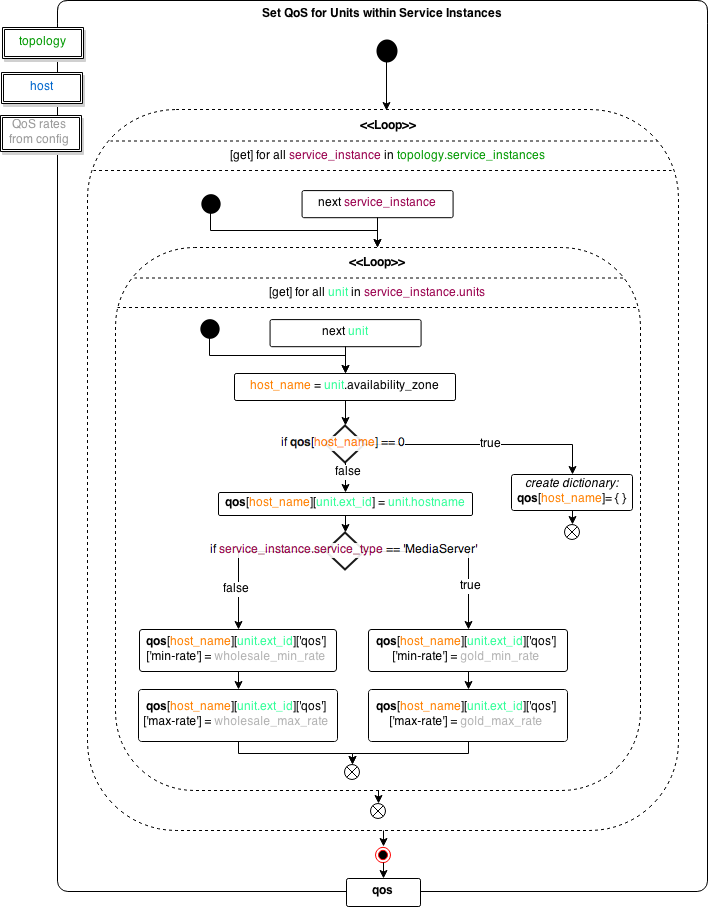
\includegraphics[width=0.6\textwidth]{images/implementation/cm_set_qos.png}

\caption{Method for setting QoS for all Units}
\end{figure}

The dictionary that this method returns is then converted to the JSON format and sent to the Connectivity Manager Agent by performing a HTTP POST to the \textit{/qoses} path of the IP address that is set for the \textit{cm\_agent\_ip} property in the configuration file.

\section{Connectivity Manager Agent - Components and Operations}

The two major operations that the Connectivity Manager needs to perform in order to provide the required services to this project is retrieving the resource status of the data center and setting QoS for the servers ports.

For using the OVS Client it needs to access the OVSDB that is located on each host. In order to allow that, the following command needs to be executed on them once:
\begin{lstlisting}[language=commands]
$ sudo ovs-vsctl set-manager ptcp:6640
\end{lstlisting}

This enables remote administration through a passive TCP connection using the local IP address and port 6640. 

\subsection{Get list of all hosts and their utilization state}

The following figure displays the way in which the CM Agent creates a dictionary containing the list of all hosts within the selected tenant. It contains information such as the amount of already running virtual machines, the amount of allocated RAM in MB and the number of vCPUs in use. For each of the virtual machines it shows their ID, name, and further resource information that is later needed for setting QoS. In case the VM already has a QoS assurance attached to its port, the corresponding minimal and maximal rates are shown.

\begin{figure}[H]
\centering

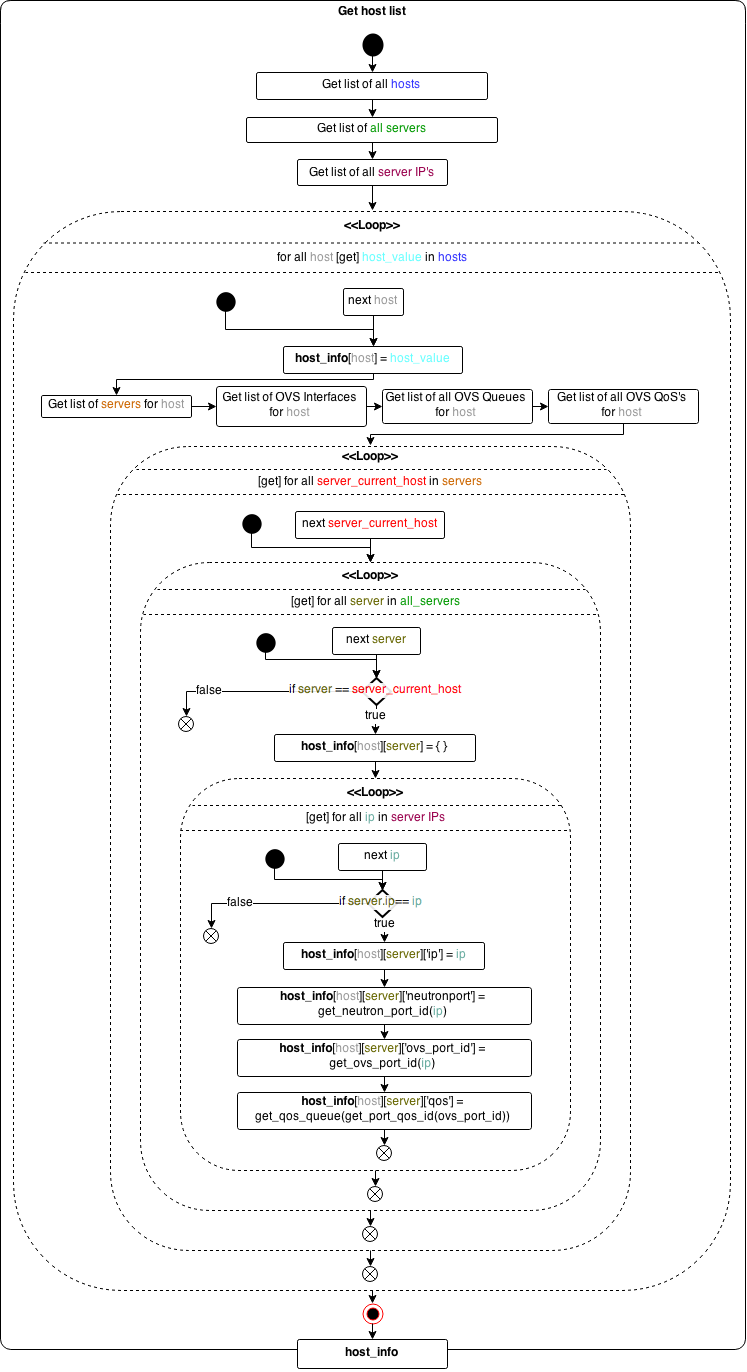
\includegraphics[width=0.65\textwidth]{images/implementation/cma_host_list}

\caption{Get list of hosts}
\end{figure}

In order to identify the rates that might have already been attached to a VM's port, a few steps need to be taken. With the server's IP address the Neutron Port ID can be retrieved. This Neutron Port ID has a Port ID within Open vSwitch that can be retrieved from the OVSDB. 

\begin{figure}[H]
\centering

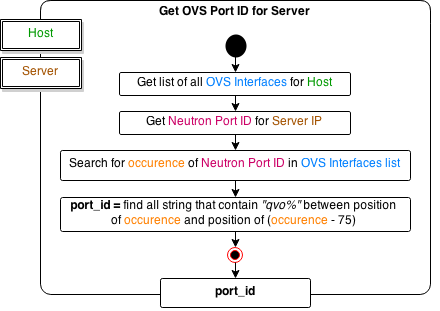
\includegraphics[width=0.5\textwidth]{images/implementation/cma_get_ovs_port_server}

\caption{Get OVS Port ID for server}
\end{figure}

Each Port contains a field for QoS, which holds its QoS ID. This ID can then be filtered from the Queue table and the associated rates are listed in there.

\begin{figure}[H]
\centering

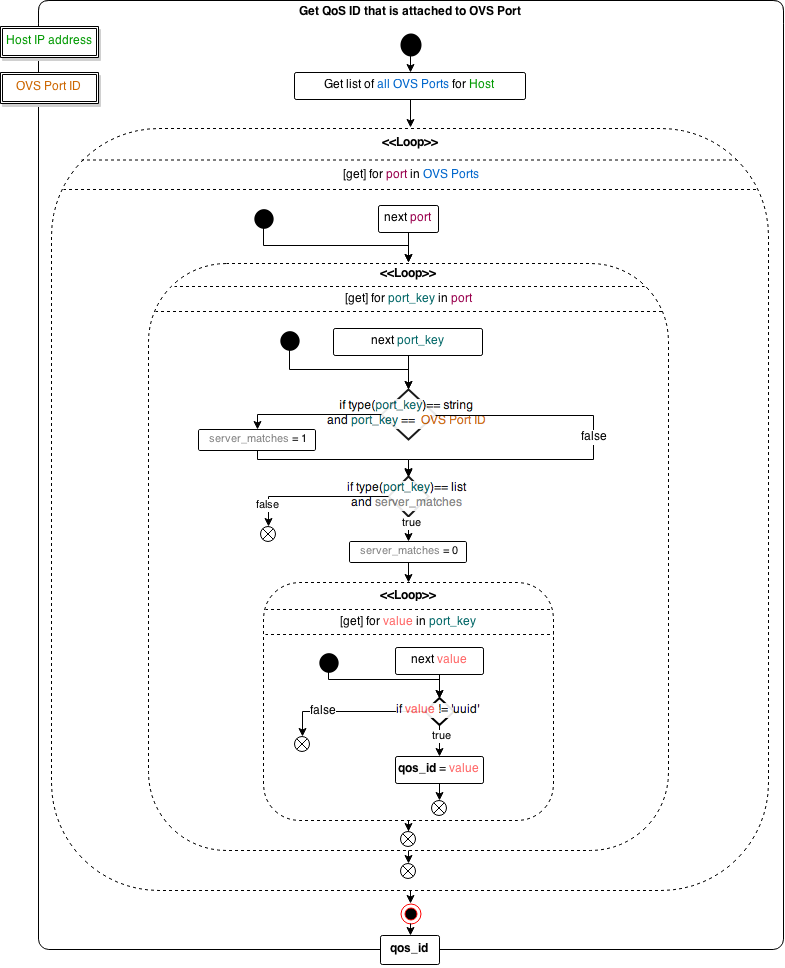
\includegraphics[width=0.7\textwidth]{images/implementation/cma_get_qos_id_for_ovs_port}

\caption{Get QoS ID for OVS Port}
\end{figure}

\subsection{Set QoS rates for all servers}

In order to set the bandwidth rates for the servers this method first retrieves the list of all hosts that was mentioned in the previous figure and description. When the \textit{Set QoS} method is called through a request to the API the method body from the HTTP POST is passed onto it. This dictionary contains all QoS rates that need to be set for each server. 


\begin{figure}[H]
\centering

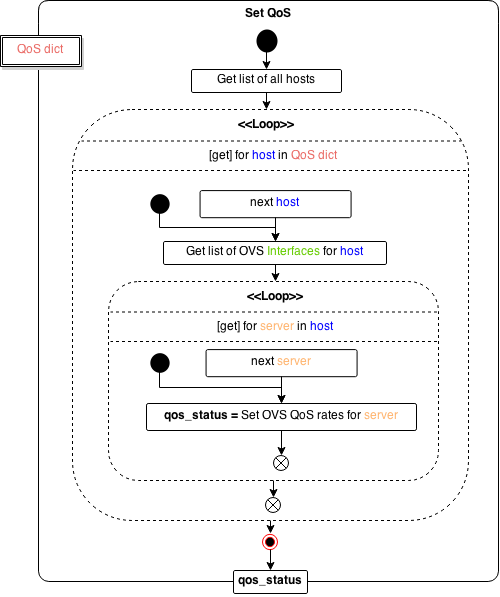
\includegraphics[width=0.5\textwidth]{images/implementation/cma_set_qos}

\caption{Set requested QoS rates for all servers}
\end{figure}

The method that is called from within the above figure for setting QoS for a single server performs the following activities:

\begin{figure}[H]
\centering

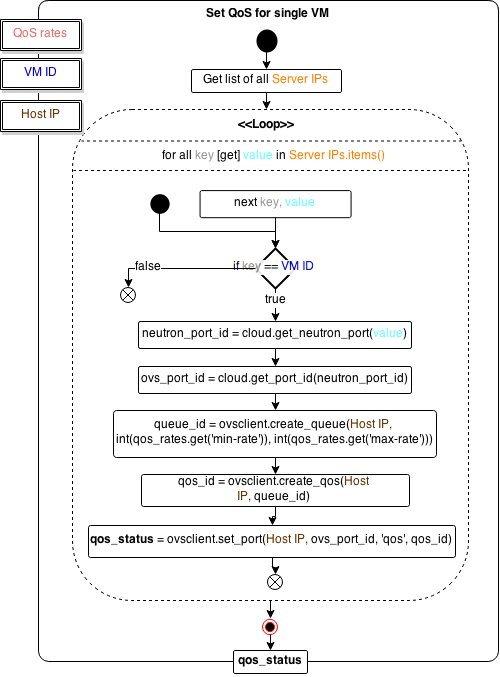
\includegraphics[width=0.4\textwidth]{images/implementation/cma_set_qos_single_server}

\caption{Set QoS rates for a single server}
\end{figure}

\subsection{API}

The API was implemented using Bottle. It is a fast, simple and lightweight WSGI micro web-framework \cite{bottle-docs}. Therein three routes were defined:
\begin{lstlisting}[language=json]
# Welcome Screen
self._app.route('/', method="GET", callback=self._welcome)
# Host method
self._app.route('/hosts', method="GET", callback=self._hosts_list)
# QoS method
self._app.route('/qoses', method=["POST", "OPTIONS"], callback=self._qoses_set)
\end{lstlisting}

The first route contains a welcome message and can be used to check if the WSGI app is currently running.
The /hosts route calls the list\_hosts() method in the Agent when a HTTP GET is received.
When the /qoses route is called with the QoS parameters in its HTTP body it calls the set\_qos() method in the Agent class.

The server uses the localhost IP address and is served and listens on port 8091. It is important that this IP address is whitelisted in case a firewall exists. In the case of using a Vagrant box the port needed to be forwarded to the local machine.

\section{Tests}

For testing the components of the Connectivity Manager Agent the code was synchronized to a local testbed with two virtual machines, one of which acted as the control node and the other just as a compute node. 

\begin{figure}[H]
\centering

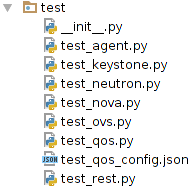
\includegraphics[width=0.17\textwidth]{images/implementation/cma_tests.png}

\caption{Connectivity Manager Agent: Test package}
\end{figure}

These functional tests contain the following methods of the main components:
\begin{itemize}
\item Agent: instantiates the Agent class and tests listing the information about all hosts
\item Keystone: tests retrieving the token and endpoint
\item Neutron: lists all ports and shows the Neutron Port ID for a selected IP address
\item Nova: retrieves all hosts and their servers
\item OVS: tests the main functionalities that are used within this work: listing all interfaces, ports, queues, qos's and creating a new queue and qos that are then attached to a OVS port
\item QoS: takes the parameters set in the \textit{test\_qos\_config.json} file as an input and posts it to the API in order to try and set QoS on the defined server ports
\item ReST: tests retrieving the list of all hosts through the API
\end{itemize}

The tests for the Connectivity Manager are part of the testing packages of the Elastic Media Manager, because that is the only way they are called. The \textit{test\_deploy.py} was used for checking if the integration works successfully.  It uses a predefined topology from a local file. The following minimized configuration was used during the tests:
\begin{lstlisting}[language=json]
{
    "name":"local_nm_template_minified",
    "service_instances": [
        {
            "name":"Controller",
            "service_type":"Controller"
        },
        {
            "name":"Broker",
            "service_type":"Broker"
        }
    ]
}
\end{lstlisting}

To find out more about the parameters that each of the service\_types corresponds to, please check the \textit{Topology Definition} % % LINK TO SECTION % %
in the Evaluation section.
\chapter{Evaluation}

\section{Feature Analysis}


\section{Connectivity Manager Integration with NUBOMEDIA project}

% % CM deliverable % %

The Connectivity Manager (CM) is part of the NUBOMEDIA platform and is placed between the virtual network resource management of the cloud infrastructure and the
multimedia application. The main focus of the CM is related to management and control of network functions of the virtual network infrastructure provided by OpenStack.

Nubomedia is an elastic Platform-as-a-Service (PaaS) cloud for interactive social multimedia \cite{nubomedia}. Its architecture is based on media pipelines: chains of elements providing media capabilities such as encryption, transcoding, augmented reality or video content analysis. These chains allow building arbitrarily complex media processing for applications. As a unique feature, from the point of view of the pipelines, the NUBOMEDIA cloud infrastructure behaves as a single virtual super-computer encompassing all the available resources of the underlying physical network.

\section{Network Performance Analysis}

The following section contains information about the used configuration and then different scenarios that were used to evaluate the effectiveness of the Connectivity Manager. All scenarios used the same topology and were run on a tenant without any other deployed servers or stacks. The bandwidth tests were performed using the iperf tool.

\subsection{Test-bed Configuration}

The testbed consists of two nodes with the following hardware characteristics:

\begin{tabularx}{\textwidth}{ |X|X|X|X| }
\hline Name & \textbf{Controller node} & \textbf{Compute node} \\ 
\hline Hostname & datacenter-4 & dc4-comp \\ 
\hline OS & Ubuntu 14.04.1 LTS & Ubuntu 14.04.1 LTS \\ 
\hline RAM & 12 GB & 8 GB \\ 
\hline CPU & 8-core Intel Core i7-4765T CPU @ 2.00GHz & 4-core Intel(R) Core(TM) i3-2120T CPU @ 2.60GHz \\ 
\hline Ethernet card & Intel Corporation Gigabit Ethernet Connection I217-LM & Intel Corporation 82579LM Gigabit Network Connection \\ 
\hline 
\end{tabularx}

The two nodes are connected to a Gigabit-Ethernet switch. The installation of OpenStack was performed using the devstack script as outlined in section ... (Implementation / Devstack) .

\subsection{Installation of Connectivity Manager Agent}

A setup script exists in order to make it easier to get the CM Agent running. It builds installs all the necessary Python packages in a virtual environment, in order to have all packages isolated from the already existing Python set-up. This ensures that all packages are in the required version and don't interfere with the ones that are needed OpenStack or other applications. 

First of all the git repository needs to be cloned from the remote git server. For the installation the cm-agent.sh script needs to be executed with the 'install' option.
\begin{lstlisting}
stack@datacenter-4:~/nubomedia$ ./cm-agent.sh 
Usage: cm-agent.sh option
options:
  install   - install the server
  update    - updates the server
  start     - start the server
  uninstall - uninstall the server
  clean     - remove build files
\end{lstlisting}
The installation process includes setting up the virtual environment, installing all required Python packages and copying the configuration file to the /etc/nubomedia folder.

The configuration file needs to be customized, so it contains the IP address of the controller node and the correct OpenStack credentials:
\begin{lstlisting}
stack@datacenter-4:~$ cat /etc/nubomedia/cm-agent.properties 
os_username=admin
os_password=pass
os_auth_url=http://192.168.41.45:5000/v2.0
os_tenant=demo
\end{lstlisting}

Lastly it can be run in a screen session using the following command: \\
\textit{\$ venv/bin/python cm-agent/wsgi/application.py}

\subsection{Topology Definition}

The topology that is used for the evaluation contains the following services instances:
\begin{lstlisting}
data/json_file/topologies/topology_local.json:
{
    "name":"local_nm_template_minified",
    "service_instances": [
        {
            "name":"Controller",
            "service_type":"Controller"
        },
        {
            "name":"Broker",
            "service_type":"Broker"
        },
        {
            "name":"MediaServer",
            "service_type":"MediaServer"
        }
    ]
}
\end{lstlisting}

It can be deployed using a test application which performs a HTTP POST to the EMM API at the \textit{/topologies} path.

The service types are further defined in another JSON file, which includes their configuration, networks and other parameters that are needed for provisioning. As one example the Media Server service is given below:

\begin{lstlisting}
data/json_file/services/MediaService.json 
{
    "service_type": "MediaServer",
    "version":"1",
    "image": "trusty-iperf",
    "flavor": "m1.mini",
    "key":"nubomedia",
    "configuration": {
    },
    "size": {
        "min": 1,
        "def": 3,
        "max": 5
    },
    "networks": [
        {
            "name":"Network-1",
            "private_net":"8048fd67-70a6-447d-a779-8a86f9eeb35d",
            "private_subnet": "0df3f54c-d1af-4b82-8376-18baa11d0e98",
            "public_net": "62024eab-23c2-4a81-a996-87af4d252282",
            "security_groups": [
                "SecurityGroup-MediaServer"
            ]
        }
    ],
    "requirements": [
        {
            "name":"$BROKER_IP",
            "parameter":"private_ip",
            "source":"Broker",
            "obj_name": "Network-1"
        }
    ]
}
\end{lstlisting}

\subsection{Scenario 1: Without Instance Placement Engine \& QoS enabled}

In this first scenario the deployment without any influence of the Connectivity Manager is shown. Here Nova randomly decides about the placement of the servers. In this case 4 servers were placed on the control node and one server on the compute node.

\begin{figure}[H]
\centering

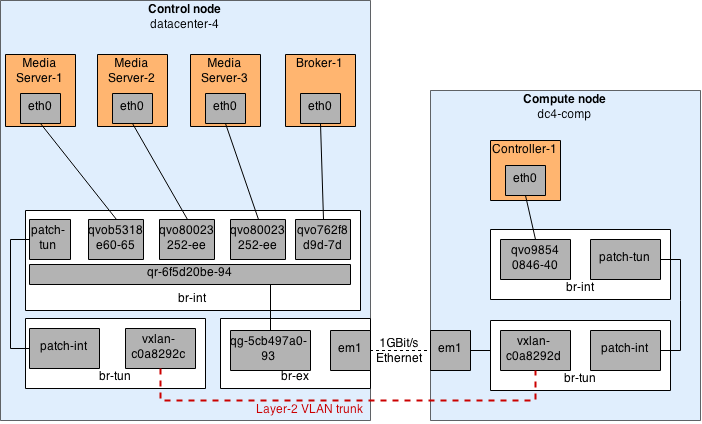
\includegraphics[width=0.7\textwidth]{images/evaluation/testbed_scenario1}

\caption{Scenario 1: Placement of servers without Connectivity Manager}
\end{figure}

For testing the bandwidth the MediaServer-2 was used as a TCP server using iperf. All other servers connected to it in client mode sending and retrieving TCP packets in a timeframe of 10 seconds. The following graph shows the bandwidth usage of the servers.

\begin{figure}[H]
\centering

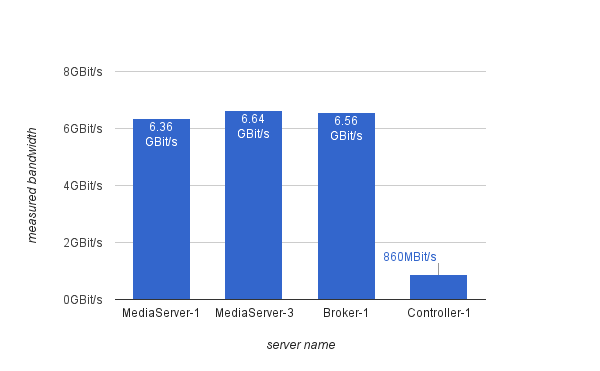
\includegraphics[width=0.5\textwidth]{images/evaluation/testbed_scenario1_bw}

\caption{Scenario 1: Bandwidth comparison}
\end{figure}

As visible the network performance of the server on the separate node performs much worse, which is also due to the fact that there is only a Gigabit-Ethernet connection between the nodes.

\subsection{Scenario 2: With Instance Placement Engine enabled, but without QoS}

In this next scenario, the Instance Placement Engine was enabled and therefore the availability zone in the topology was successfully set to a single host.

\begin{figure}[H]
\centering

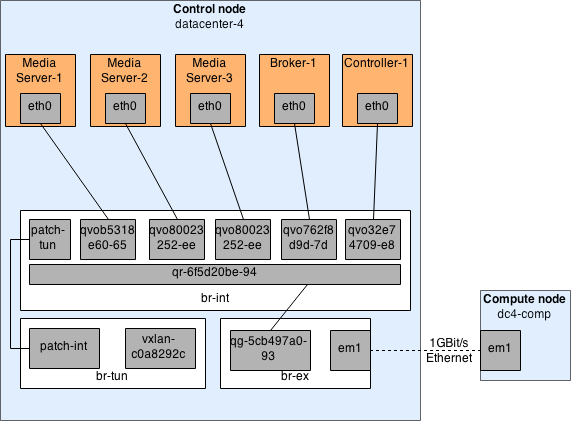
\includegraphics[width=0.7\textwidth]{images/evaluation/testbed_scenario2}

\caption{Scenario 2: Placement of servers with Connectivity Manager}
\end{figure}

The following graph shows that the available bandwidth is now evenly distributed for all servers. However the traffic of the MediaServers should be prioritized, which is why QoS is needed to further improve the connectivity according to the requirements.

\begin{figure}[H]
\centering

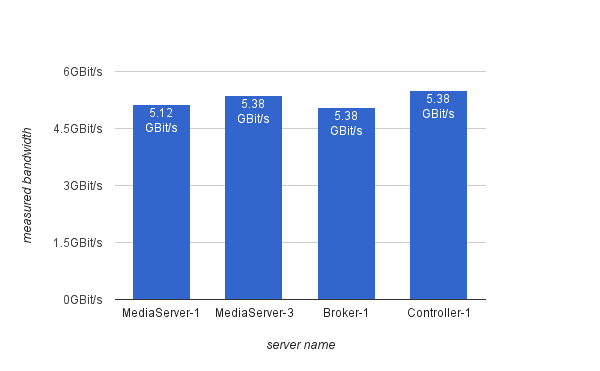
\includegraphics[width=0.5\textwidth]{images/evaluation/testbed_scenario2_bw}

\caption{Scenario 2: Bandwidth comparison}
\end{figure}


\subsection{Scenario 3: Instance Placement Engine and QoS Manager enabled}

The servers are again placed on a single host and the Quality of Service configuration that was previously set in the configuration is applied. All media servers have a guaranteed bandwidth rate of 100 MBit/s and a maximum rate of 10 GBit/s, while all servers of other instance types have a rate between 100 MBit/s and 1 GBit/s.

\begin{figure}[H]
\centering

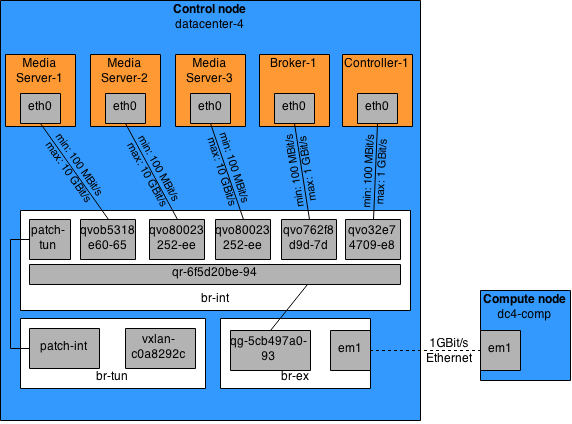
\includegraphics[width=0.7\textwidth]{images/evaluation/testbed_scenario3}

\caption{Scenario 3: Placement of servers using the Connectivity Manager with QoS enabled}
\end{figure}

For this last scenario two servers were set as iperf-servers and three servers as iperf-clients. The \textit{'Controller-1'} server acted as the server for a connection with the \textit{'MediaServer-2'} while the \textit{'MediaServer-3'} received packets from \textit{'MediaServer-1'} and \textit{'Broker-1'}.

The topology with it's configured QoS Queues is also visible by performing a HTTP GET to the Connectivity Manager Agent at the /hosts path:
\begin{lstlisting}
{  
   "dc4-comp":{  
      "cpu_total":4,
      "ip":"192.168.41.44",
      "servers":{  

      },
      "instances":0,
      "ram_total":7788,
      "ram_used":0,
      "cpu_used":0,
      "id":2
   },
   "datacenter-4":{  
      "cpu_total":8,
      "ip":"192.168.41.45",
      "servers":{  
         "9a2b6c59-72fd-4576-8a51-27c506b77980":{  
            "ip":"10.0.0.15",
            "ovs_port_id":"qvob5318e60-65",
            "qos":{  
               "queues":{  
                  "0":{  
                     "rates":{  
                        "max-rate":"10000000000",
                        "min-rate":"100000000"
                     },
                     "uuid":"e9183562-fe04-4341-99e0-8a3b73659101"
                  }
               },
               "uuid":"b3a0edc0-60bc-4c06-ac5a-6219a2add194"
            },
            "name":"MediaServer-1",
            "neutron_port":"b5318e60-6534-4f80-ab05-8d4747f1022a"
         },
         "6b2f58f6-4cc7-4438-b6bf-2af54f13f0ec":{  
            "ip":"10.0.0.13",
            "ovs_port_id":"qvo58137c93-bc",
            "qos":{  
               "queues":{  
                  "0":{  
                     "rates":{  
                        "max-rate":"10000000000",
                        "min-rate":"100000000"
                     },
                     "uuid":"86ed41aa-b48d-47fa-805a-6eab61d23948"
                  }
               },
               "uuid":"9b3794a1-7046-4f9d-afb6-0e13a4bbd2d5"
            },
            "name":"MediaServer-3",
            "neutron_port":"58137c93-bc56-4ddd-8330-8af161bc3e3d"
         },
         "45aecdb2-75ee-4876-af69-4793a7d4c242":{  
            "ip":"10.0.0.17",
            "ovs_port_id":"qvo80023252-ee",
            "qos":{  
               "queues":{  
                  "0":{  
                     "rates":{  
                        "max-rate":"10000000000",
                        "min-rate":"100000000"
                     },
                     "uuid":"e8e6fdf1-62c3-42ca-a354-6437bf7eb9f2"
                  }
               },
               "uuid":"241d9954-2048-4b00-bdfc-14c9c5191151"
            },
            "name":"MediaServer-2",
            "neutron_port":"80023252-ee83-4205-9503-7e86a16d7286"
         },
         "dedd78db-2be4-4655-b08a-8cac40087823":{  
            "ip":"10.0.0.16",
            "ovs_port_id":"qvo762f8d9d-7d",
            "qos":{  
               "queues":{  
                  "0":{  
                     "rates":{  
                        "max-rate":"1000000000",
                        "min-rate":"100000000"
                     },
                     "uuid":"8b0f7fbb-e511-46ee-b20d-eb7b0f0a5c18"
                  }
               },
               "uuid":"edcfcbb5-1bfc-4797-a101-845ceb55bc1c"
            },
            "name":"Broker-1",
            "neutron_port":"762f8d9d-7d7f-45fb-836b-eaa3ebaad71b"
         },
         "1eb23d4c-fb5a-42eb-9943-2fb2585b8c04":{  
            "ip":"10.0.0.14",
            "ovs_port_id":"qvo32e74709-e8",
            "qos":{  
               "queues":{  
                  "0":{  
                     "rates":{  
                        "max-rate":"1000000000",
                        "min-rate":"100000000"
                     },
                     "uuid":"81d2a604-bc78-41fd-a3ac-71c550251286"
                  }
               },
               "uuid":"db182f5b-afba-4163-9ca5-51501aed1959"
            },
            "name":"Controller-1",
            "neutron_port":"32e74709-e812-4f14-bbd9-2e9926fa1377"
         }
      },
      "instances":5,
      "ram_total":11813,
      "ram_used":3072,
      "cpu_used":5,
      "id":1
   }
}
\end{lstlisting}

\begin{figure}[H]
\centering

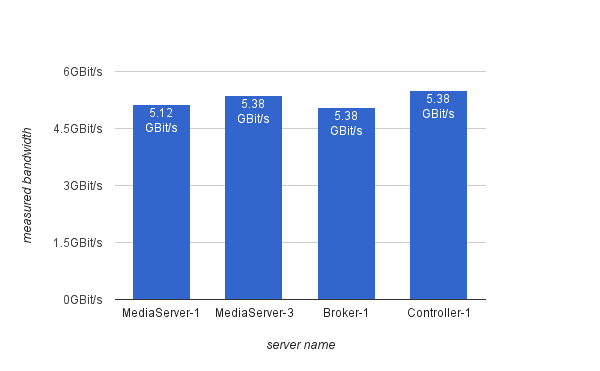
\includegraphics[width=0.5\textwidth]{images/evaluation/testbed_scenario2_bw}

\caption{Scenario 3: Bandwidth comparison}
\end{figure}

The first two bars show that the egress port on the Open vSwitch that the \textit{'MediaServer-3'} is connected to is limited to a combined bandwidth of 10 GBit/s. This is why the two connections share the available bandwidth and are nearly equal. It has to be remarked that the network performance is the average of a 10-second bandwidth test.

In the other QoS class the \textit{'MediaServer-2'} which is connecting to \textit{'Controller-1'} uses almost the full bandwidth of the available 1 GBit/s.

\section{Conclusion}

The three test scenarios show an improvement of the network performance, which is given through placing the servers on a single host. Additionally with enabling Quality of Service, the network bandwidth is shaped according to the requirements. It has been shown that the connection of MediaServers is prioritized to the connection of servers of other service instance types. The Service-Level-Agreement of the Gold and Wholesale classes are fulfilled.
 \cleardoublepage
\chapter{Conclusion}

\section{Summary}

With the use of SDN and OpenFlow, a framework for creating programmable networks already exists. However the integration of an SDN Controller can further extend the capabilities of SDN in OpenStack. By default, the network bandwidth supplied to different servers is on a best-effort basis and topologies that are deployed using the orchestration service Heat cannot be placed on specific hosts. The work described in this thesis explains how these limitations can be overcome. With the help of the Open vSwitch configuration tool it is possible to get information about the current state of the switched network and enable QoS using Queues. The required configuration and information can now be accessed through an API. The Elastic Media Manager is able to access this information and make decisions about where the topology has the best-performing network connectivity. The bandwidth rates according to their Service-Level Agreements can be easily updated and extended. The evaluation gives a step-by-step explanation of the improvements in bandwidth rates with the use of the Connectivity Manager in relation to the requirements.

\section{Problems Encountered}

One significant problem during the development process was getting a stable test-bed running with the correct configuration. Devstack helped significantly in this regard, because aside from adjusting the configuration file, not many manual corrections needed to be made. However some of the features that are in the 'stable' version of OpenStack Juno still need further bug-fixing and cannot currently be used in a production environment. During the testing of various state-of-the-art solutions, a significant amount of time was spent on testing different versions, which was unsuccessful. Due to the significant time taken, comparisons to other solutions for enabling Quality of Service could not be evaluated. 

\section{Future Work}

For future development, the algorithm for selecting the best-performing host could take more dynamic factors into account. One possibility is to check the network speed of all the host's network interfaces. Furthermore, it would be a good approach to implement the features of the Connectivity Manager Agent as a Neutron extension and make use of the existing Neutron API. The implementation of QoS could be based on the existing blueprint and be shared with the OpenStack community to achieve an integration into the Neutron repository.

Additional, one further step that could be evaluated for Quality of Service is to perform Flow modifications, as opposed to the currently used procedure of attaching the Queue to the OVS Port and having a rate-limit on the egress traffic. With this approach, the ingress traffic for a specific Port could be filtered with enqueuing and then set as the Flow action. 

\protect \addtocontents{toc}{\protect\newpage}  % Seitenumbruch im Inhaltsverzeichnis
\cleardoublepage


% Erstes Literaturverzeichnis, ohne BibTeX

\interlinepenalty=10000 % Literatureintr�ge: Abs�tze zusammenhalten
\cleardoublepage
\addcontentsline{toc}{chapter}{Bibliography}   
%F�r das nachfolgende exemplarische Literaturverzeichnis wurde die einfache thebibliography-Umgebung von Latex verwendet. F�r Studien- und Diplomarbeiten mit weniger als 40 Quellen sollte diese auf jeden Fall ausreichen und hat gegen�ber dem komplexen Bibtex-Paket weiterhin den Vorteil flexiblerer Formatierungsm�glichkeiten.
%
%Im Anschluss an das exemplarische Literaturverzeichnis ist ein zweites Verzeichnis beigef�gt, welches weiterf�hrende Quellen zum vorliegenden Latex-Template enth�lt: Download-Links zur Software, freie Online-Latex-Handb�cher usw.



\begin{thebibliography}{Ti}



\bibitem[1]{roadtosdn} N. Feamster, J. Rexford, E. Zegura: \glqq The Road to SDN\grqq, ACM Queue, Volume 11, Issue 12, December 30, 2013.
\bibitem[2]{onfnewnorm} Open Networking Foundation: \glqq Software-Defined Networking: The New Norm For Networks \grqq, ONF White Paper, April 13, 2012.
\bibitem[3]{onfdefinition} Open Networking Foundation: \glqq Software-Defined Networking (SDN) Definition \grqq, \url{https://www.opennetworking.org/sdn-resources/sdn-definition}
\bibitem[4]{ofversion13} S. Natarajan, SDN Hub: \glqq OpenFlow version 1.3 tutorial \grqq, \url{http://sdnhub.org/tutorials/openflow-1-3/}
\bibitem[5]{ofspecification} Open Networking Foundation: \glqq OpenFlow Switch Specification \grqq, Version 1.3.0, June 25, 2012.
\bibitem[6]{ovs-faq} Open vSwitch: \glqq Open vSwitch - Frequently Asked Questions \grqq, \url{http://git.openvswitch.org/cgi-bin/gitweb.cgi?p=openvswitch;a=blob_plain;f=FAQ;hb=HEAD}
\bibitem[7]{ovs-readme} Open vSwitch: \glqq Open vSwitch - Readme \grqq, \url{https://github.com/openvswitch/ovs/blob/master/README.md}
\bibitem[8]{prognetworkingovs} J. Gross, VMware: \glqq Programmable Networking with Open vSwitch \grqq, LinuxCon, September, 2013. \url{https://events.linuxfoundation.org/sites/events/files/slides/OVS-LinuxCon\%202013.pdf}
\bibitem[9]{ovsdeepdive} J. Pettit, E. Lopez, VMware: \glqq OpenStack: OVS Deep Dive \grqq, 07 November, 2013.
\bibitem[10]{ovsdbmanual} Open vSwitch: \glqq Open vSwitch Manual\grqq, \url{http://openvswitch.org/ovs-vswitchd.conf.db.5.pdf}
\bibitem[11]{tc-manual} B. Hubert: \glqq tc - Linux man page\grqq, \url{http://linux.die.net/man/8/tc}
\bibitem[12]{htb-guide} M. Devera, D. Cohen: \glqq HTB Linux queuing discipline manual\grqq, \url{http://luxik.cdi.cz/~devik/qos/htb/manual/userg.htm}
GRE: \url{http://www.juniper.net/documentation/en_US/junos14.1/topics/concept/gre-tunnel-services.html}

\end{thebibliography}





\begin{appendix}

\chapter{Glossar}
\label{anhang_e}



\textcolor{darkred}{Anmerkung: Das vorliegende Glossar wurde ohne die Zuhilfenahme der speziellen Glossarumgebungen von Latex erstellt, um eine etwas freiere Formatierung nutzen zu k�nnen.}
\medskip



\interlinepenalty=10000 % keine Schusterjungen, keine Hurenkinder



\begin{description}

\item[\bf{2,5D-Datensatz}] $\rightarrow$Tiefenbild.

\item[\bf{3D-Modell, 3D-Modellerfassung (optische)}] Der Begriff des 3D-Modells wird in der vorliegenden Arbeit f�r wasserdichte Oberfl�chenmodelle verwendet. Dies dient zur Abgrenzung gegen�ber 3D-Volumenmodellen und $\rightarrow$Tiefenbildern. Der Begriff der Optischen 3D-Modellerfassung umschlie�t hier neben der eigentlichen Sensordatenauswertung auch die $\rightarrow$3D-Registrierung und die Schritte der Nachbearbeitung wie Gl�tten und Ausd�nnen der Daten und Stiching-Operationen.

\item[\bf{3D-Registrierung}] Vgl. Abschnitte 2.4, 4.3 und $\rightarrow$Registrierung.

\end{description}
\interlinepenalty=100



                    % E
\end{appendix}






% Zweites Literaturverzeichnis, mit BibTeX

%\renewcommand\bibname{Weiterf�hrende Literatur zu wissenschaftlichen Ausarbeitungen}
%\nocite{*} % auch die nicht verwendeten bibtex-Eintr�ge einblenden
%\cleardoublepage
%\addcontentsline{toc}{chapter}{Weiterf�hrende Literatur zu wissenschaftlichen Ausarbeitungen}
%\bibliography{bibliografie}
%\interlinepenalty=100



% Sachverzeichnis einf�gen

%\renewcommand\indexname{Sachverzeichnis}
%\cleardoublepage
%\addcontentsline{toc}{chapter}{Sachverzeichnis}
%\linespread{0.99} % Abhilfe zu Schusterjungen .. im Index. Die Zahl ist entspr zu variieren
%\printindex                                 



% Schmutzblatt (leere Seite am Ende)

\newpage                                    
\pagestyle{empty}
\begin{figure}[H]
\centering

\includegraphics[width=0.9\textwidth]{images/general/leer.jpg}
\end{figure}



\end{document}




















%
